\section{Casi d'uso} 
\subsection{Attori dei casi d'uso}
\subsubsection{Attori primari}
\begin{figure}[h]
	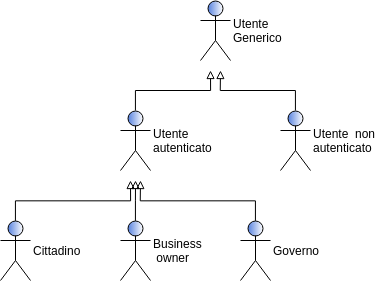
\includegraphics[width=7cm]{res/images/attori_primari.png}
	\centering
	\caption{Gerarchia degli attori primari}
\end{figure}
\begin{description}[style=nextline]
	\item[Utente generico]
	Si riferisce ad un utente generico che accede alla piattaforma dal sito web.
	\item[Utente non autenticato]
	Si riferisce ad un utente generico che non ha ancora effettuato l'autenticazione alla piattaforma.
	\item[Utente autenticato]
	Si riferisce ad un utente generico che si è autenticato nel sistema con la procedura di login. Ciò implica che sia in possesso di una chiave\glosp valida sulla rete. Ethereum\glosp con la quale, precedentemente, ha portato a termine la procedura di autenticazione.
	\item[Cittadino] Si riferisce ad un utente che si è autenticato nel sistema con il ruolo di cittadino.
	\item[Azienda] Si riferisce ad un utente che si è autenticato nel sistema con il ruolo di azienda. Le azioni sono eseguite considerando l'azienda come persona giuridica, nonostante le azioni vengano eseguite da un suo rappresentante.
	\item[Governo\glosp] Si riferisce ad un utente che si è autenticato al sistema con il ruolo di governo\glo. Nelle parti successive del documento tale parola verrà intesa con tale significato.
\end{description}
\subsubsection{Attori secondari}
\begin{description}[style=nextline]
	\item[MetaMask]
	Plug-in\glosp per browser che permette di interfacciarsi con la rete Ethereum\glosp e di validare le transazioni con la propria chiave privata.
	
\end{description}

\subsection{Elenco dei casi d'uso}
In questa sezione vi sono elencati tutti i casi d'uso individuati. Ogni caso d'uso rappresenta uno scenario per uno o più attori, ovviamente applicabile anche ad eventuali attori derivati. Ogni caso d'uso, inoltre, viene descritto tramite diagrammi dei casi d'uso e possiede una precondizione seguita da una postcondizione.
\subsubsection*{Operazioni utenti}
Di seguito sono riportati tutti i casi d'uso che coinvolgono come attore primario l'utente generico, l'utente non autenticato, l'utente autenticato, il cittadino e parte dei casi d'uso che coinvolgono l'azienda.

\begin{figure}[H]
	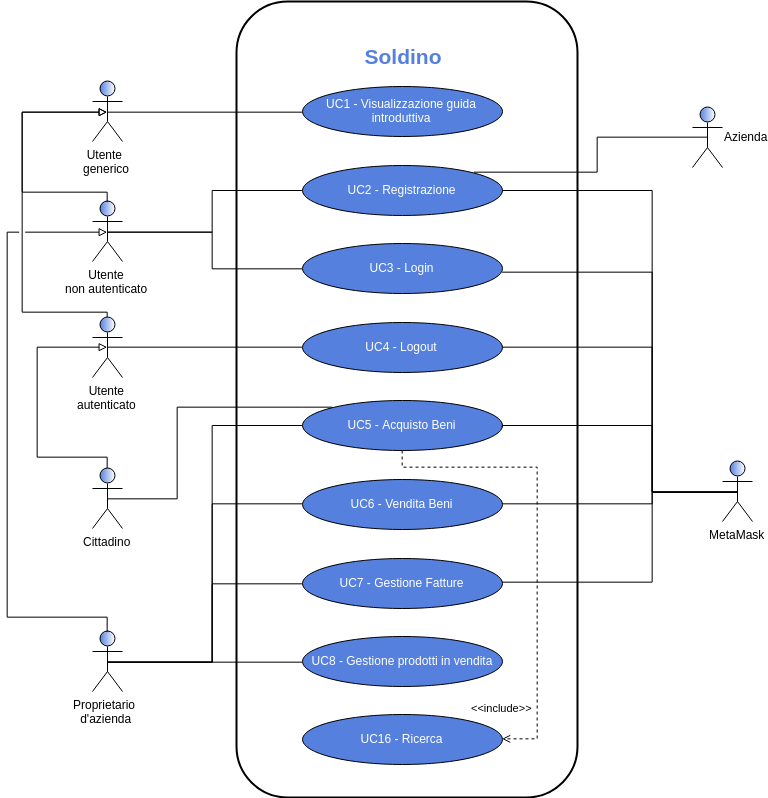
\includegraphics[width=14cm]{res/images/UseCase1-8.png}
	\centering
	\caption{Use Cases che interessano gli utenti}
\end{figure}
\begin{figure}[h]
	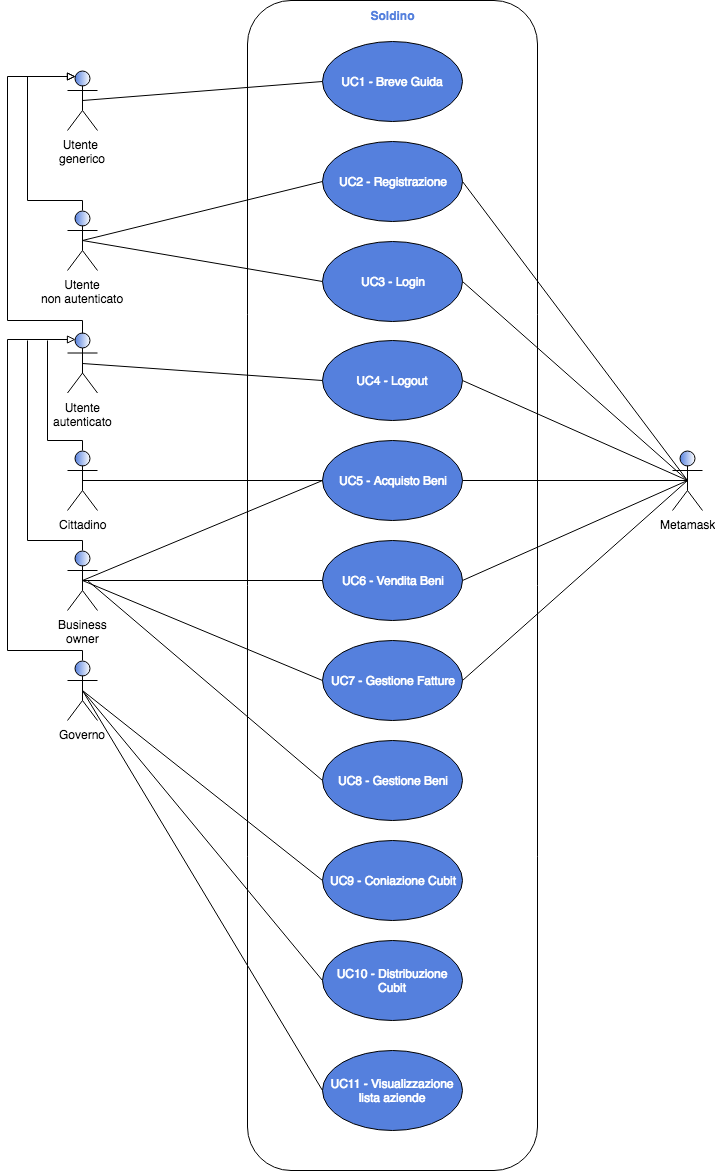
\includegraphics[width=9.38cm]{res/images/Elenco_casi_d_uso.png}
	\centering
	\caption{Elenco dei casi d'uso}
\end{figure}
\subsubsection{UC1 - Breve Guida}
\begin{itemize}
	\item \textbf{Attori Primari}: utente generico;
	\item \textbf{Descrizione}: l'utente visualizza una guida riguardante l'installazione ed il funzionamento del plug-in Metamask\glosp. Viene spiegato come impostare le chiavi del plug-in e come utilizzarlo per accedere al sistema;
	\item \textbf{Scenario principale}: l'utente accede alla guida;
	\item \textbf{Precondizione}: il sistema è raggiungibile e funzionante, l'utente desidera ricevere delle informazioni per imparare ad autenticarsi alla piattaforma;
	\item \textbf{Postcondizione}: il sistema fornisce all'utente, attraverso la lettura della guida, tutte le istruzioni necessarie alla registrazione ed all'autenticazione.
	
	
\end{itemize}
\subsubsection{UC2 - Registrazione}
\begin{figure}[h]
	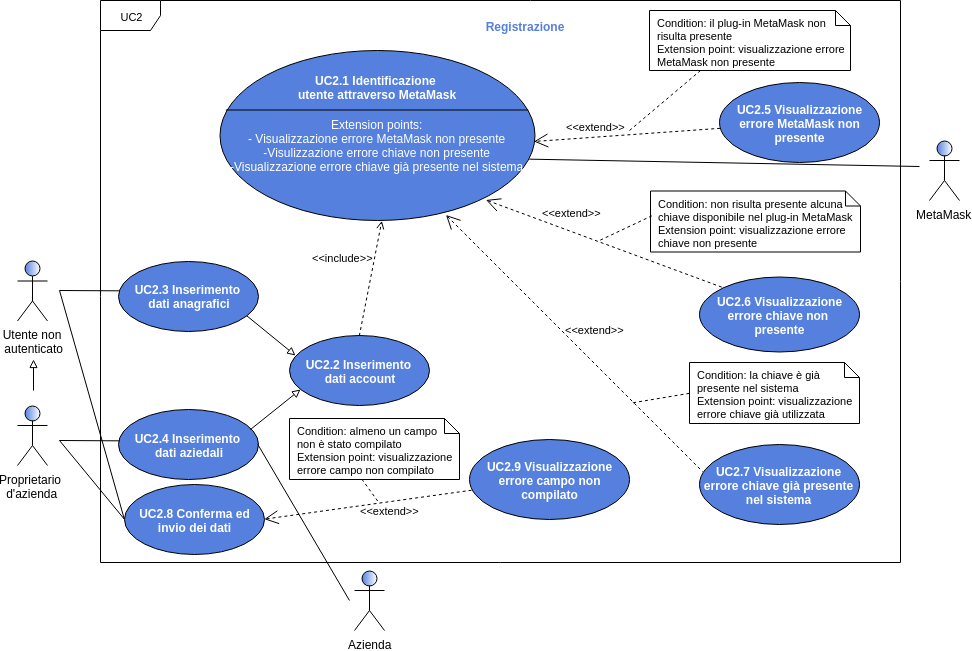
\includegraphics[width=16cm]{res/images/UC2Registrazione.png}
	\centering
	\caption{UC2 - Registrazione}
\end{figure}
\begin{itemize}
	\item \textbf{Attori Primari}: utente non autenticato, eventualmente proprietario d'azienda;
	\item \textbf{Attori Secondari}: MetaMask\glosp;
	\item \textbf{Descrizione}: l'utente non autenticato compila tutti i campi richiesti al fine di registrarsi sulla piattaforma, successivamente dovrà aspettare che il proprio account venga verificato da parte del governo\glosp;
	\item \textbf{Scenario}: 
	
	\begin{enumerate}[label=\alph*.]
		
		\item l'utente vuole registrarsi come normale \textbf{cittadino}: 
		\begin{enumerate}[label=\roman*.]
			\item l'utente inserisce i dati anagrafici [UC2.3];
			\item l'utente conferma ed invia i dati inseriti [UC2.8].
		\end{enumerate}
		
		
		\item l'utente vuole registrare la propria \textbf{azienda}:
		\begin{enumerate}[label=\roman*.]
			\item l'utente inserisce i dati aziendali [UC2.4];
			\item l'utente conferma ed invia i dati inseriti [UC2.8].
		\end{enumerate}
		
		
		
	\end{enumerate}
	\item \textbf{Precondizione}: l'utente ha il plug-in MetaMask\glosp installato e correttamente impostato sul proprio browser, viene considerato dal sistema come un utente non autenticato e desidera registrarsi come cittadino o registrare la propria azienda; 
	\item \textbf{Postcondizione}: il sistema riceve le informazioni dell'utente, le salva ed inoltra la richiesta di verifica ed approvazione al governo\glosp.
	
\end{itemize}
\subsubsection{UC2.1 - Identificazione utente attraverso MetaMask\glosp}
\begin{itemize}
	\item \textbf{Attori Primari}: utente non autenticato;
	\item \textbf{Attori Secondari}: MetaMask\glosp;
	\item \textbf{Descrizione}: il sistema verifica la presenza del plug-in MetaMask\glosp, al quale richiede la chiave pubblica che l'utente desidera usare come identificativo e metodo di pagamento. Essendo la chiave univoca, il sistema controlla che nessun utente registrato stia attualmente utilizzandola. Il sistema mostra infine l'interfaccia contente il form di registrazione;
	\item \textbf{Scenario}: il sistema, prima di mostrare il form per la registrazione, controlla la presenza di una chiave\glosp utilizzabile attraverso il plug-in MetaMask\glosp.
	\item \textbf{Estensioni}:
	\begin{itemize}
		\item \textbf{UC2.5}: se il plug-in MetaMask\glosp non risulta installato nel browser dell'utente, o è stato disabilitato, esso viene avvisato tramite l'apposito messaggio di errore;
		\item \textbf{UC2.6}: se l'utente non possiede una chiave\glosp su MetaMask\glosp, esso viene avvisato tramite l'apposito messaggio di errore;
		\item \textbf{UC2.7}: se è presente una chiave su MetaMask\glosp, ma il sistema rileva che essa è già stata utilizzata per la registrazione sulla piattaforma, allora l'utente viene avvisato attraverso l'apposito messaggio di errore.
	\end{itemize}
	\item \textbf{Precondizione}: l'utente ha cliccato sul link per accedere al form di registrazione di un account cittadino o aziendale;
	\item \textbf{Postcondizione}: il sistema ha verificato che la chiave\glosp con la quale l'utente sta cercando di registrarsi non risulti già utilizzata nel sistema. La chiave è salvata e verrà utilizzata durante la registrazione. All'utente è permesso compilare i dati relativi alla tipologia di registrazione richiesta.
	
\end{itemize}
\subsubsection{UC2.2 - Inserimento dati account}
\begin{figure}[h]
	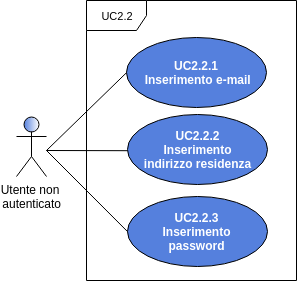
\includegraphics[width=8cm]{res/images/UC2-2RegistrazioneGenerale.png}
	\centering
	\caption{UC2-2 Inserimento dati account}
\end{figure}
\begin{itemize}
	\item \textbf{Attori Primari}: utente non autenticato;
	\item \textbf{Descrizione}: l'utente compila il form contenente i dati relativi all'account;
	\item \textbf{Scenario}: l'utente compila tutti i campi del form riguardanti l'account, ovvero:
	\begin{enumerate}[label=\alph*.]
		\item l'utente inserisce l'email da associare all'account [UC2.2.1];
		\item l'utente inserisce l'indirizzo di residenza da associare all'account [UC2.2.2];
		\item l'utente inserisce la password da associare all'account [UC2.2.3].
	\end{enumerate}
	\item \textbf{Specializzazione}:
	\begin{itemize}
		\item \textbf{UC2.3}: l'utente inserisce i dati relativi alla registrazione di un cittadino;
		\item \textbf{UC2.4}: l'utente inserisce i dati relativi alla registrazione di un'azienda.
		
	\end{itemize}
	\item \textbf{Precondizione}: l'utente ha espresso la volontà di iscriversi alla piattaforma cliccando uno dei link per la registrazione. Il sistema ha rilevato e salvato una chiave\glosp valida attraverso il plug-in MetaMask\glosp;
	\item \textbf{Postcondizione}: l'utente ha compilato i campi relativi ai dati dell'account.
	
\end{itemize}
\subsubsection{UC2.2.1 - Inserimento e-mail}
\begin{itemize}
	\item \textbf{Attori Primari}: utente non autenticato;
	\item \textbf{Descrizione}: al fine di portare a termine il processo di registrazione l'utente deve inserire un indirizzo e-mail, campo ritenuto obbligatorio;
	\item \textbf{Scenario}: l'utente compila il campo relativo all'indirizzo e-mail;
	\item \textbf{Precondizione}: il sistema ha reso disponibile il campo per l'inserimento dell'indirizzo e-mail;
	\item \textbf{Postcondizione}: l'utente ha compilato il campo con la propria e-mail.
	
\end{itemize}
\subsubsection{UC2.2.2 - Inserimento indirizzo di residenza}
\begin{itemize}
	\item \textbf{Attori Primari}: utente non autenticato;
	\item \textbf{Descrizione}: al fine di portare a termine il processo di registrazione l'utente deve inserire un indirizzo di residenza, campo ritenuto obbligatorio;
	\item \textbf{Scenario}: l'utente compila il campo relativo all'indirizzo di residenza;
	\item \textbf{Precondizione}: il sistema ha reso disponibile il campo per l'inserimento dell'indirizzo di residenza;
	\item \textbf{Postcondizione}: l'utente ha compilato il campo con l'indirizzo relativo alla residenza.
\end{itemize}
\subsubsection{UC2.2.3 - Inserimento password}
\begin{itemize}
	\item \textbf{Attori Primari}: utente non autenticato;
	\item \textbf{Descrizione}: al fine di portare a termine il processo di registrazione l'utente deve inserire una password, campo ritenuto obbligatorio;
	\item \textbf{Scenario}: l'utente compila il campo relativo alla password;
	\item \textbf{Precondizione}: il sistema ha reso disponibile il campo per l'inserimento della password;
	\item \textbf{Postcondizione}: l'utente ha compilato il campo con la password scelta.
\end{itemize}
\subsubsection{UC2.3 - Inserimento dati anagrafici}
\begin{figure}[h]
	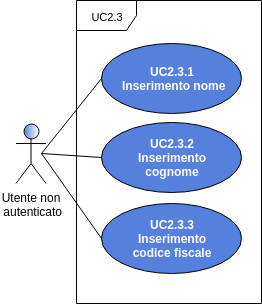
\includegraphics[width=6cm]{res/images/UC2-3Registrazione-cliente.png}
	\centering
	\caption{UC2.3 - Registrazione cittadino}
\end{figure}
\begin{itemize}
	\item \textbf{Attori Primari}: utente non autenticato;
	\item \textbf{Descrizione}: l'utente compila i campi relativi alla registrazione alla piattaforma come cittadino;
	\item \textbf{Scenario}: l'utente ha cliccato sul pulsante di registrazione di un cittadino, il sistema rende disponibile il form di registrazione relativo e l'utente compila tutti i campi necessari;
	\item \textbf{Precondizione}: l'utente ha espresso la volontà di iscriversi alla piattaforma cliccando il link per la registrazione come cittadino. Il sistema ha rilevato e salvato una chiave\glosp valida attraverso il plug-in MetaMask\glosp;
	\item \textbf{Postcondizione}: l'utente ha compilato i campi relativi alla registrazione di un cittadino alla piattaforma.
\end{itemize}
\subsubsection{UC2.3.1 - Inserimento nome}
\begin{itemize}
	\item \textbf{Attori Primari}: utente non autenticato;
	\item \textbf{Descrizione}: al fine di portare a termine il processo di registrazione di un nuovo cittadino, l'utente deve inserire il proprio nome;
	\item \textbf{Scenario}: l'utente compila il campo relativo al nome;
	\item \textbf{Precondizione}: il sistema ha reso disponibile il campo per l'inserimento del nome;
	\item \textbf{Postcondizione}: l'utente ha compilato il campo con il proprio nome.
\end{itemize}
\subsubsection{UC2.3.2 - Inserimento cognome}
\begin{itemize}
	\item \textbf{Attori Primari}: utente non autenticato;
	\item \textbf{Descrizione}: al fine di portare a termine il processo di registrazione di un nuovo cittadino, l'utente deve inserire il proprio cognome;
	\item \textbf{Scenario}: l'utente compila il campo relativo al cognome;
	\item \textbf{Precondizione}: il sistema ha reso disponibile il campo per l'inserimento del cognome;
	\item \textbf{Postcondizione}: l'utente ha compilato il campo con il proprio cognome.
\end{itemize}
\subsubsection{UC2.3.3 - Inserimento codice fiscale}
\begin{itemize}
	\item \textbf{Attori Primari}: utente non autenticato;
	\item \textbf{Descrizione}: al fine di portare a termine il processo di registrazione di un nuovo cittadino, l'utente deve inserire il proprio codice fiscale;
	\item \textbf{Scenario}: l'utente compila il campo relativo al codice fiscale;
	\item \textbf{Precondizione}: il sistema ha reso disponibile il campo per l'inserimento del codice fiscale;
	\item \textbf{Postcondizione}: l'utente ha compilato il campo con il proprio codice fiscale.
\end{itemize}
\subsubsection{UC2.4 - Inserimento dati aziendali}
\begin{figure}[h]
	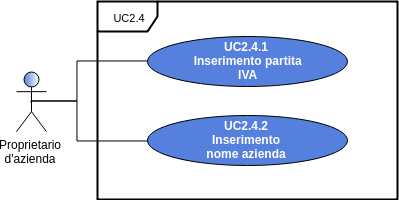
\includegraphics[width=6cm]{res/images/UC2-4RegistrazioneAzienda.png}
	\centering
	\caption{UC2 - Registrazione di un'azienda}
\end{figure}
\begin{itemize}
	\item \textbf{Attori Primari}: proprietario d'azienda;
	\item \textbf{Attori Secondari}: azienda;
	\item \textbf{Descrizione}: l'utente compila i campi relativi alla registrazione della propria azienda sulla piattaforma;
	\item \textbf{Scenario}: l'utente ha cliccato sul pulsante di registrazione di un'azienda, il sistema rende disponibile il form di registrazione relativo e l'utente compila tutti i campi necessari;
	\item \textbf{Precondizione}: l'utente ha espresso la volontà di iscriversi alla piattaforma cliccando il link per la registrazione di un'azienda. Il sistema ha rilevato e salvato una chiave\glosp valida attraverso il plug-in MetaMask\glosp;
	\item \textbf{Postcondizione}: l'utente ha compilato i campi relativi alla registrazione di un'azienda alla piattaforma.
\end{itemize}
\subsubsection{UC2.4.1 - Inserimento partita IVA}
\begin{itemize}
	\item \textbf{Attori Primari}: proprietario d'azienda;
	\item \textbf{Descrizione}: al fine di portare a termine il processo di registrazione della propria azienda, l'utente deve inserire la relativa partita IVA;
	\item \textbf{Scenario}: l'utente compila il campo relativo alla partita IVA;
	\item \textbf{Precondizione}: il sistema ha reso disponibile il campo per l'inserimento della partita IVA;
	\item \textbf{Postcondizione}: l'utente ha compilato il campo con la partita IVA dell'azienda che intende registrare.
\end{itemize}
\subsubsection{UC2.4.2 - Inserimento nome azienda}
\begin{itemize}
	\item \textbf{Attori Primari}: proprietario d'azienda;
	\item \textbf{Descrizione}: al fine di portare a termine il processo di registrazione della propria azienda, l'utente deve inserire il relativo nome aziendale;
	\item \textbf{Scenario}: l'utente compila il campo relativo al nome aziendale;
	\item \textbf{Precondizione}: il sistema ha reso disponibile il campo per l'inserimento del nome aziendale;
	\item \textbf{Postcondizione}: l'utente ha compilato il campo con il nome dell'azienda che intende registrare.
\end{itemize}



\subsubsection{UC2.5 - Visualizzazione errore MetaMask\glosp non presente}
\begin{itemize}
	\item \textbf{Attori Primari}: utente non autenticato
	\item \textbf{Descrizione}: l'utente visualizza un errore relativo al fatto che non il plug-in MetaMask\glosp non risulta installato o attualmente disabilitato;
	\item \textbf{Scenario}: l'utente non ancora identificato dal sistema tenta di accedere a sezioni che necessitano la presenza di MetaMask\glosp, e quest'ultimo non è installato o attualmente disabilitato;
	\item \textbf{Precondizione}: MetaMask\glosp non è presente nel browser dell'utente o è attualmente disabilitato;
	\item \textbf{Postcondizione}: l'utente è a conoscenza che è necessario attivare o installare MetaMask\glosp per proseguire.
	
\end{itemize}

\subsubsection{UC2.6 - Visualizzazione errore chiave non 
	presente}
\begin{itemize}
	\item \textbf{Attori Primari}: utente non autenticato;
	\item \textbf{Attori Secondari}: MetaMask\glosp;
	\item \textbf{Descrizione}:
	l'utente visualizza un messaggio di errore relativo al fatto che non è stata rilevata nessuna chiave\glosp all'interno del plug-in MetaMask\glosp;
	\item \textbf{Scenario}: l'utente tenta di accedere ad una sezione del sito che necessita l'identificazione di una chiave\glosp attraverso il plug-in MetaMask\glosp, e questo non contiene almeno una chiave\glosp;
	\item \textbf{Precondizione}: il plug-in MetaMask\glosp è correttamente configurato, ma non è presente nessuna chiave\glosp;
	\item \textbf{Postcondizione}:
	l'utente è consapevole che il plug-in MetaMask\glosp non contiene almeno una chiave\glosp.
	
\end{itemize}




\subsubsection{UC2.7 - Visualizzazione errore chiave già presente nel sistema}
\begin{itemize}
	\item \textbf{Attori Primari}: utente non autenticato;
	\item \textbf{Attori Secondari}: MetaMask\glosp;
	\item \textbf{Descrizione}:
	l'utente visualizza un messaggio di errore relativo al fatto che la chiave\glosp prelevata dal plug-in MetaMask\glosp risulta già presente nella piattaforma;
	\item \textbf{Scenario}: l'utente tenta di registrarsi al sito utilizzando una chiave\glosp già presente nel sistema;
	\item \textbf{Precondizione}: MetaMask\glosp è correttamente configurato, ma la chiave\glosp selezionata nel plug-in è già stata utilizzata nella piattaforma;
	\item \textbf{Postcondizione}:
	l'utente è consapevole che la chiave\glosp selezionata nel plug-in MetaMask\glosp è già stata utilizzata nella piattaforma, e quindi che necessita di un'altra chiave per effettuare la nuova registrazione.
\end{itemize}

\subsubsection{UC2.8 - Conferma ed invio dei dati}
\begin{itemize}
	\item \textbf{Attori Primari}: utente non autenticato, eventualmente proprietario d'azienda;
	\item \textbf{Descrizione}:
	l'utente preme il pulsante per la conferma e l'invio dei dati. A schermo viene mostrato un messaggio che conferma il successo dell'operazione e spiega di attendere la verifica da parte del governo\glosp prima di poter effettivamente accedere alla piattaforma.
	\item \textbf{Scenario}: l'utente preme il pulsante di verifica ed invio dei dati dopo aver compilato i campi del form;
	\item \textbf{Estensioni}: 
	\begin{itemize}
		\item \textbf{UC2.9}: l'utente preme il pulsante di verifica senza aver compilato almeno uno dei campi del form, viene visualizzato il relativo errore;
	\end{itemize}
	\item \textbf{Precondizione}: il sistema permette all'utente di compilare il form di registrazione. \`E presente il pulsante per la conferma dei dati;
	\item \textbf{Postcondizione}:
	l'utente è consapevole che la richiesta di registrazione è avvenuta con successo ed è consapevole del fatto che dovrà attendere la verifica dell'account da parte del governo\glosp.
\end{itemize}

\subsubsection{UC2.9 - Visualizzazione errore campo non compilato}
\begin{itemize}
	\item \textbf{Attori Primari}: utente non autenticato;
	\item \textbf{Descrizione}:
	l'utente visualizza un messaggio di errore relativo al fatto che almeno uno dei campi del form di registrazione risulta non compilato;
	\item \textbf{Scenario}: l'utente tenta di confermare i dati della registrazione senza aver compilato tutti i dati del form;
	\item \textbf{Precondizione}: il sistema permette all'utente di compilare il form di registrazione. \`E presente il pulsante per la conferma dei dati;
	\item \textbf{Postcondizione}:
	l'utente è consapevole che per inviare i dati e terminare la procedura di registrazione deve compilare tutti i campi presenti nel form.
\end{itemize}

\begin{figure}[h]
	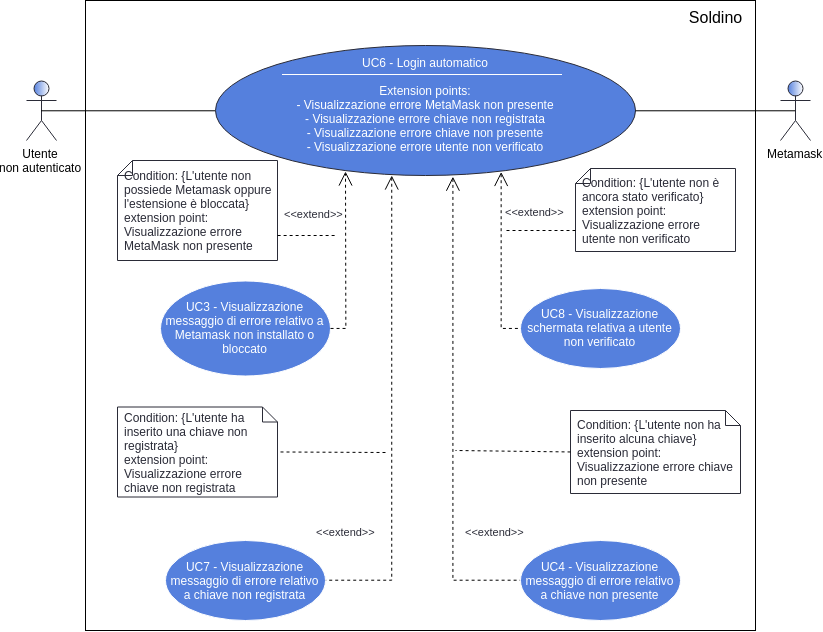
\includegraphics[width=12cm]{res/images/login.png} %da adattare in larghezza
	\centering
	\caption{UC3 - Login ed errori annessi}
	
\end{figure}
\subsubsection{UC6 - Login automatico}
\begin{itemize}
	\item \textbf{Attori Primari}:
	utente non autenticato;
	\item \textbf{Attori Secondari}:
	MetaMask\glo;
	\item \textbf{Descrizione}:
	in modo automatico, il sistema procede all'identificazione dell'utente;
	\item \textbf{Scenario principale}:
	l'utente non ancora autenticato richiede il login;
	\item \textbf{Estensioni}:
	\begin{itemize}
		\item \textbf{UC2.5}: se l'utente non dispone di MetaMask\glosp o ha disabilitato l'estensione, viene visualizzato un messaggio di errore a riguardo;
		\item \textbf{UC2.6}: se l'utente non possiede una chiave\glosp su MetaMask\glo, esso viene avvisato tramite l'apposito messaggio di errore;
		\item \textbf{UC3.2}: se l'utente tenta di accedere al sito tramite MetaMask\glosp senza aver mai provveduto a registrarsi, riceverà un messaggio di errore a riguardo;
		
		\item \textbf{UC3.3}: se l'utente si è registrato ma il suo account è stato disabilitato, riceverà un messaggio di errore a riguardo.
	\end{itemize}
	\item \textbf{Precondizione}:
	l'utente tenta di autenticarsi alla piattaforma;
	\item \textbf{Postcondizione}:
	l'utente si è autenticato con successo, ed è stato identificato dal sistema nel ruolo di cittadino, azienda o utente governativo. A seconda della tipologia di utente vengono rese disponili diverse pagine e funzionalità.
\end{itemize}
\subsubsection{UC7 - Visualizzazione messaggio di errore relativo a chiave non registrata}
\begin{itemize}
	\item \textbf{Attori Primari}:
	utente non autenticato;
	\item \textbf{Descrizione}:
	l'utente visualizza un messaggio di errore dovuto al fatto che ha tentato il login senza essersi registrato in precedenza;
	\item \textbf{Scenario principale}:
	l'utente tenta di eseguire la procedura di login alla piattaforma senza essere registrato;
	\item \textbf{Precondizione}:
	l'utente tenta di autenticarsi nella piattaforma;
	\item \textbf{Postcondizione}: viene visualizzato un messaggio d'errore per informare l'utente del fatto che è necessario registrarsi alla piattaforma prima di poter poi effettuare la procedura di login.
\end{itemize}
\subsubsection{UC8 - Visualizzazione schermata relativa a utente non abilitato}
\begin{itemize}
	\item \textbf{Attori Primari}: utente non autenticato;
	\item \textbf{Descrizione}:
	l'utente tenta di autenticarsi alla piattaforma, tuttavia, a causa della disabilitazione del suo account, il login viene interrotto, e l'utente visualizza il messaggio personalizzato lasciato dal governo che illustra la causa della disabilitazione dell'account;
	\item \textbf{Scenario principale}:
	l'utente non autenticato con account disabilitato tenta di autenticarsi. La procedura di autenticazione viene bloccata a causa dello stato dell'account;
	\item \textbf{Precondizione}:
	un utente non autenticato, registrato alla piattaforma e con account disabilitato tenta di effettuare il login automatico;
	\item \textbf{Postcondizione}:  viene visualizzato un messaggio d'errore per informare l'utente del fatto che il proprio account è stato disabilitato dal governo. Se quest'ultimo, durante la procedura di disabilitazione, ha inserito un messaggio contenente la causa di tale azione, allora tale messaggio viene visualizzato.
\end{itemize}
\begin{figure}[h]
	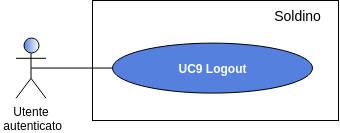
\includegraphics[width=6cm]{res/images/UC9-Logout.png} %da adattare in larghezza
	\centering
	\caption{UC9-Logout}
	
\end{figure}
\subsubsection{UC9 - Logout}
\begin{itemize}
	\item \textbf{Attori Primari}:
	utente autenticato;
	\item \textbf{Attori Secondari}:
	MetaMask\glo;
	\item \textbf{Descrizione}: l'utente richiede il logout dalla piattaforma web. Vengono visualizzate le informazioni necessarie per procedere alla procedura di logout, che deve essere effettuata attraverso l'utilizzo del plug-in MetaMask\glo;
	\item \textbf{Scenario principale}: l'utente è autenticato dal sito e richiede di effettuare il logout, premendo sull'apposito pulsante;
	\item \textbf{Precondizione}: l'utente ha effettuato il login alla piattaforma web e richiede di essere disconnesso dal sito;
	\item \textbf{Postcondizione}: vengono visualizzate le istruzioni necessarie per eseguire il logout tramite MetaMask\glo. 
\end{itemize}


 \subsubsection{UC5 - Visualizzazione beni}
 \begin{figure}[h]
 	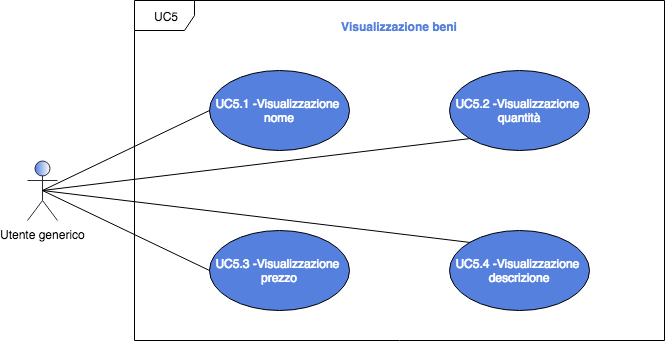
\includegraphics[width=10cm]{res/images/UC5VisualizzazioneBeni.png}
 	\centering
 	\caption{UC5 - Visualizzazione beni}
 \end{figure}
 \begin{itemize}
 	\item \textbf{Attori Primari}: utente autenticato;
 	\item \textbf{Descrizione}: l'utente visualizza una lista dettagliata di informazioni relative ad un bene o servizio;
 	\item \textbf{Scenario}: l'utente si trova all'interno della pagina di un bene o servizio e può trarre le seguenti informazioni:
 		\begin{enumerate}[label=\alph*.]
 		\item visualizzazione nome [UC5.1];
 		\item visualizzazione quantità [UC5.2];
 		\item visualizzazione prezzo [UC5.3];
 		\item visualizzazione descrizione [UC5.4];
 	\end{enumerate}
 	\item \textbf{Precondizione}: l'utente, navigando nel sito, risulta all'interno della pagina di un bene o servizio;
 	\item \textbf{Postcondizione}: l'utente può procedere all'acquisto del bene o del servizio, se loggato.
 \end{itemize}
 \subsubsection{UC5.1 - Visualizzazione nome}
\begin{itemize}
	\item \textbf{Attori Primari}: utente autenticato;
	\item \textbf{Descrizione}: l'utente visualizza il nome del bene o del servizio;
	\item \textbf{Scenario}: l'utente si trova all'interno della pagina di un bene o servizio;
	\item \textbf{Precondizione}: l'utente ha espresso la volontà di visualizzare la pagina di un bene o un servizio;
	\item \textbf{Postcondizione}: l'utente conosce il nome del prodotto.
\end{itemize}
 \subsubsection{UC5.2 - Visualizzazione quantità}
\begin{itemize}
	\item \textbf{Attori Primari}: utente autenticato;
	\item \textbf{Descrizione}: l'utente visualizza la quantità del bene o del servizio selezionato;
	\item \textbf{Scenario}: l'utente si trova all'interno della pagina di un bene o servizio;
	\item \textbf{Precondizione}: l'utente ha espresso la volontà di visualizzare la pagina di un bene o un servizio;
	\item \textbf{Postcondizione}: l'utente è consapevole del fatto che la quantità visualizzata saà quella che, se vorrà, inserirà nel carrello.
\end{itemize}
 \subsubsection{UC5.3 - Visualizzazione prezzo}
\begin{itemize}
	\item \textbf{Attori Primari}: utente autenticato;
	\item \textbf{Descrizione}: l'utente visualizza il prezzo del bene o del servizio;
	\item \textbf{Scenario}: l'utente si trova all'interno della pagina di un bene o servizio;
	\item \textbf{Precondizione}: l'utente ha espresso la volontà di visualizzare la pagina di un bene o un servizio;
	\item \textbf{Postcondizione}: l'utente conosce il prezzo del prodotto.
\end{itemize}
 \subsubsection{UC5.4 - Visualizzazione descrizione}
\begin{itemize}
	\item \textbf{Attori Primari}: utente autenticato;
	\item \textbf{Descrizione}: l'utente visualizza la descrizione del bene o del servizio;
	\item \textbf{Scenario}: l'utente si trova all'interno della pagina di un bene o servizio;
	\item \textbf{Precondizione}: l'utente ha espresso la volontà di visualizzare la pagina di un bene o un servizio;
	\item \textbf{Postcondizione}: l'utente conosce la descrizione del prodotto.
\end{itemize}
\subsubsection{UC6 - Gestione carrello}
 \begin{figure}[h]
	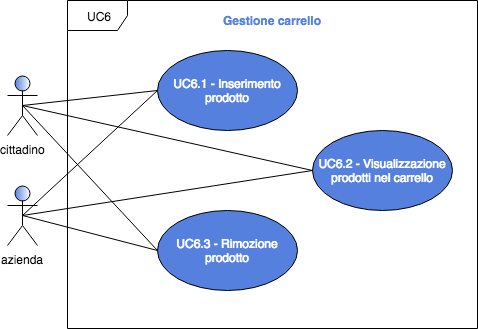
\includegraphics[width=6cm]{res/images/UC6GestioneCarrello.png}
	\centering
	\caption{UC6 - Gestione carrello}
\end{figure}
\begin{itemize}
	\item \textbf{Attori Primari}: cittadino, azienda;
	\item \textbf{Descrizione}: ai cittadini ed alle aziende è reso disponibile un carrello virtuale per poter organizzare i propri acquisti;
	\item \textbf{Scenario principale}: l'utente effettua le operazioni necessarie all'acquisto di beni e servizi. Esse comprendono:
	\begin{enumerate}[label=\alph*.]
		\item l'inserimento di un bene/servizio [UC6.1];
		\item la visualizzazione dei prodotti nel carrello [UC6.2];
		\item la modifica della quantità relativa ad un prodotto nel carrello [UC6.3];
		\item la rimozione di un prodotto dal carrello [UC6.4].
	\end{enumerate}
	\item \textbf{Precondizione}: il sistema riconosce l'utente come cittadino o azienda e rende disponibile il carrello virtuale;
	\item \textbf{Postcondizione}: l'utente può procedere all'acquisto di tutti i beni e/o servizi presenti nel carrello.
\end{itemize} 
 \subsubsection{UC6.1 - Inserimento prodotto}
\begin{itemize}
	\item \textbf{Attori Primari}: cittadino, azienda;
	\item \textbf{Descrizione}: l'utente inserisce il prodotto selezionato nel carrello, nella quantità desiderata;
	\item \textbf{Scenario principale}:
	\begin{enumerate}[label=\alph*.]
		\item l'utente sta visualizzando i prodotti offerti [UC5];
		\item l'utente seleziona la quantità desiderata del prodotto [UC5.1];
		\item l'utente preme il pulsante per l'inserimento del prodotto nel carrello.
	\end{enumerate}
	\item \textbf{Precondizione}: l'utente sta visualizzando i prodotti in vendita nella piattaforma dalla pagina dedicata;
	\item \textbf{Postcondizione}: nel carrello dell'utente è presente il bene o il servizio selezionato.
\end{itemize}
\subsubsection{UC6.2 - Visualizzazione prodotti del carrello}
\begin{itemize}
	\item \textbf{Attori Primari}: cittadino, azienda;
	\item \textbf{Descrizione}: l'utente visualizza un riepilogo di tutti i prodotti presenti all'interno del proprio carrello. Per ognuno di essi può visualizzare dei dettagli riassuntivi, che sono:
	\begin{itemize}
		\item il nome;
		\item la quantità;
		\item il prezzo unitario.
	\end{itemize}
	Inoltre è disponibile il prezzo totale dei prodotti.

	\item \textbf{Scenario principale}: l'utente si trova all'interno della pagina del proprio carrello virtuale e può visualizzare la lista dei prodotti aggiunti al carrello;
	\item \textbf{Precondizione}: l'utente deve essere all'interno della pagina del proprio carrello;
	\item \textbf{Postcondizione}: l'utente ha potuto controllare la lista dei prodotti all'interno del proprio carrello.
\end{itemize}

\subsubsection{UC6.3 - Modifica quantità di un prodotto nel carrello}
\begin{itemize}
	\item \textbf{Attori Primari}: cittadino, azienda;
	\item \textbf{Descrizione}: l'utente modifica la quantità di un prodotto presente nel proprio carrello;
	\item \textbf{Scenario principale}: l'utente si trova all'interno della pagina del proprio carrello e modifica la quantità di un prodotto, utilizzando gli appositi pulsanti di incremento e decremento della quantità;
	\item \textbf{Precondizione}: l'utente deve accedere alla pagina relativa al proprio carrello ed avervi inserito almeno un prodotto;
	\item \textbf{Postcondizione}: la quantità del prodotto considerato è stata modificata come indicato dall'utente.
\end{itemize}

\subsubsection{UC6.4 - Rimozione prodotto}
\begin{itemize}
	\item \textbf{Attori Primari}: cittadino, azienda;
	\item \textbf{Descrizione}: l'utente rimuove il prodotto selezionato dal proprio carrello;
	\item \textbf{Scenario principale}: l'utente si trova all'interno della pagina del proprio carrello e clicca sul pulsante dedicato alla rimozione di un prodotto;
	\item \textbf{Precondizione}: l'utente deve accedere alla pagina relativa al proprio carrello;
	\item \textbf{Postcondizione}: nel carrello dell'utente non è più presente il bene/servizio rimosso.
\end{itemize}
\subsubsection{UC7 - Acquisto beni}
\begin{figure}[h]
	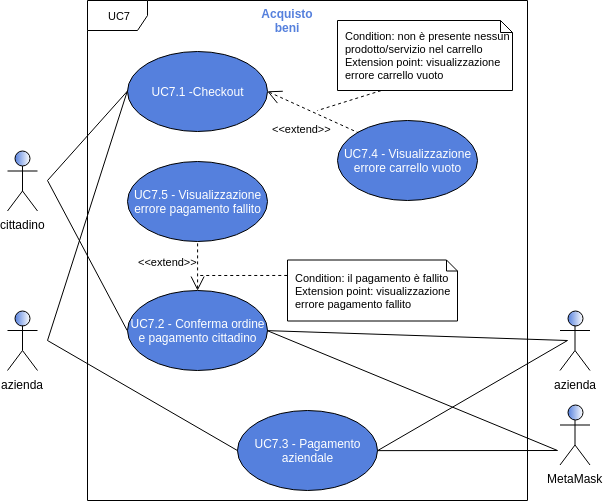
\includegraphics[width=14cm]{res/images/UC7-Generale.png}
	\centering
	\caption{UC7 - Acquisto beni}
\end{figure}
\begin{itemize}
	\item \textbf{Attori Primari}: cittadino e azienda-cliente;
	\item \textbf{Attori Secondari}: azienda-venditrice, MetaMask\glo;
	\item \textbf{Descrizione}: i cittadini e le aziende possono acquistare i prodotti/servizi che avevano precedentemente aggiunto nel carrello;
	\item \textbf{Scenario}: l'utente innanzitutto inserisce dei prodotti nel carrello [UC6.1]. Dunque procede al checkout [UC7.1] dei prodotti nel carrello:
	\begin{itemize}
		\item i cittadini procedono con la conferma dell'ordine ed il pagamento immediato [UC7.2];
		\item le aziende invece dovono scegliere un metodo di pagamento [UC7.3.1] tra il pagamento immediato [UC7.3.2] ed il pagamento dilazionato [UC7.3.3]. A differenza dei cittadini, devono successivamente approvare la proposta d'ordine dal proprio account per ottenere la fatturazione.
	\end{itemize}
	
	\item \textbf{Precondizione}: il sistema ha reso disponibile all'utente l'utilizzo del carrello per poter effettuare degli acquisti. L'utente ha inserito degli oggetti nel carrello ed ha espresso la volontà di acquistare tali prodotti;
	\item \textbf{Postcondizione}: è stato effettuato l'acquisto dei beni presenti nel carrello. Se l'utente è cittadino, allora l'ordine è concluso e viene effettuato il pagamento all'azienda venditrice. Viceversa, nel caso il cliente fosse un'azienda, viene inviata una proposta d'ordine nella pagina dedicata, che dovrà successivamente essere confermata. Inoltre, nel caso questo fosse un ordine con pagamento immediato, il sistema provvederà a trattenere i soldi dovuti all'azienda venditrice finché non verrà confermata la correttezza della proposta della fattura.
\end{itemize} 
\subsubsection{UC7.1 - Checkout}
\begin{itemize}
	\item \textbf{Attori Primari}: cittadino, azienda;
	\item \textbf{Descrizione}: l'utente effettua il checkout per poter poi acquistare i prodotti inseriti nel carrello;
	\item \textbf{Scenario}: l'utente preme il pulsante per effettuare il checkout;
	\item \textbf{Inclusioni}: 
	\begin{itemize}
		\item \textbf{UC7.6}: l'utente inserisce l'indirizzo di spedizione;
	\end{itemize}
	\item \textbf{Estensioni}: 
	\begin{itemize}
		\item \textbf{UC7.4}: l'utente preme il pulsante di checkout senza aver ancora inserito almeno un prodotto/servizio nel carrello;
	\end{itemize}
	\item \textbf{Precondizione}: il sistema ha reso disponibile il carrello all'utente, identificandolo quindi come cittadino o azienda. L'utente ha espresso la volontà di procedere con il checkout premendo l'apposito pulsante;
	\item \textbf{Postcondizione}: l'utente accede alla pagina dove poter confermare l'acquisto e procedere con il pagamento.
\end{itemize}

\subsubsection{UC7.2 - Conferma ordine e pagamento cittadino}
\begin{itemize}
	\item \textbf{Attori Primari}: cittadino;
	\item \textbf{Attori Secondari}: azienda-venditrice, MetaMask\glo;
	\item \textbf{Descrizione}: l'utente visualizza il contenuto del carrello ed ha la possibilità di confermare l'ordine e procedere al pagamento che avviene attraverso l'utilizzo del plugin Metamask\glo;
	\item \textbf{Scenario}: l'utente preme il pulsante per effettuare il checkout;
	\item \textbf{Inclusioni}: 
	\begin{itemize}
		\item \textbf{UC6.2}: l'utente visualizza un riepilogo di tutti i prodotti presenti all'interno del carrello.
	\end{itemize}
	\item \textbf{Estensioni}: 
	\begin{itemize}
		\item \textbf{UC7.5}: l'utente tenta il pagamento ma l'esito non va a buon fine. La causa del fallimento dell'operazione è gestito dal plugin stesso.
	\end{itemize}
	\item \textbf{Precondizione}: il sistema ha reso disponibile il riepilogo dei prodotti con la possibilità di effettuare la conferma dell'ordine ed il pagamento. Almeno un elemento era stato inserito nel carrello; 
	\item \textbf{Postcondizione}: l'utente ha portato a termine la procedura di acquisto dei prodotti/servizi presenti nel carrello. L'azienda venditrice ha ricevuto il pagamento dal cliente e l'ordine è aggiunto alla lista delle fatture dell'azienda. Al cliente viene segnalato il successo dell'operazione.
\end{itemize}
\subsubsection{UC7.3 - Pagamento aziendale}
\begin{figure}[H]
	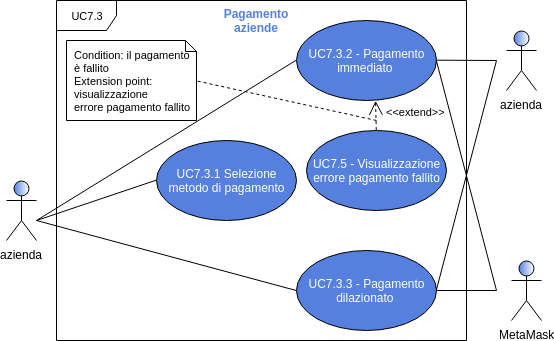
\includegraphics[width=14cm]{res/images/UC7-PagamentoAzienda.png}
	\centering
	\caption{UC7.3 - Procedura di pagamento da parte delle aziende}
\end{figure}
\begin{itemize}
	\item \textbf{Attori Primari}: azienda-cliente;
	\item \textbf{Attori Secondari}: azienda-venditrice, MetaMask\glo;
	\item \textbf{Descrizione}: le aziende hanno un processo di pagamento differente dai cittadini, possono scegliere fra pagamento immediato e dilazionato\glo;
	\item \textbf{Scenario}: l'azienda sceglie un metodo di pagamento [UC7.3.1] tra il pagamento immediato [UC7.3.2] ed il pagamento dilazionato [UC7.3.3]. Successivamente dovrà approvare la proposta d'ordine dal proprio account per ottenere la fatturazione.
	\item \textbf{Inclusioni}: 
	\begin{itemize}
		\item \textbf{UC6.2}: l'utente visualizza un riepilogo di tutti i prodotti presenti all'interno del carrello.
	\end{itemize}
	\item \textbf{Precondizione}: il sistema ha reso disponibile il riepilogo dei prodotti con la possibilità di scegliere il metodo di pagamento ed effettuare la conferma dell'ordine;
	\item \textbf{Postcondizione}: è stato scelto il metodo di pagamento e l'ordine è stato effettuato con successo. All'azienda cliente viene inviata una proposta d'ordine e vengono spiegati i passi successivi da seguire per accettare tale proposta, in maniera da validare l'ordine e ricevere la fattura.
\end{itemize} 

\subsubsection{UC7.3.1 - Selezione metodo di pagamento}
\begin{itemize}
	\item \textbf{Attori Primari}: azienda;
	\item \textbf{Descrizione}: l'utente visualizza le possibili modalità di pagamento, immediato e dilazionato\glo, seleziona uno dei due metodi e conferma la scelta;
	\item \textbf{Scenario}: l'utente seleziona una modalità di pagamento e conferma l'ordine, per poi procedere al pagamento;
	\item \textbf{Precondizione}: il sistema ha reso disponibile la scelta del metodo di pagamento e la conferma dell'ordine;
	\item \textbf{Postcondizione}: l'utente ha selezionato la modalità di pagamento per l'ordine corrente e l'ordine è stato confermato, il sistema procede con la procedura di pagamento selezionata.
\end{itemize}

\subsubsection{UC7.3.2 - Pagamento immediato}
\begin{itemize}
	\item \textbf{Attori Primari}: azienda-cliente;
	\item \textbf{Attori Secondari}: azienda-venditrice, MetaMask\glo;
	\item \textbf{Descrizione}: l'utente procede con il pagamento immediato: l'azienda-cliente versa l'importo dell'ordine nel sistema attraverso l'utilizzo del plugin MetaMask\glo. Viene inviata automaticamente la proposta d'ordine dall'azienda-venditrice all'azienda-cliente. Al cliente viene spiegato come procedere per confermare l'ordine e ricevere la fattura IVA.
	\item \textbf{Scenario}: l'utente procede con il pagamento attraverso l'ausilio del plugin MetaMask\glo;
	\item \textbf{Estensioni}: 
	\begin{itemize}
		\item \textbf{UC7.5}: l'utente tenta il pagamento ma l'esito non va a buon fine. La causa del fallimento dell'operazione è gestito dal plugin stesso.
	\end{itemize}
	\item \textbf{Precondizione}: il sistema ha reso disponibile il pagamento dell'ordine;
	\item \textbf{Postcondizione}: l'utente ha portato a termine la procedura di acquisto. Il sistema ha ricevuto il pagamento dal cliente, il cliente riceve, nella pagina dedicata, la proposta d'ordine. Al cliente viene comunicato il successo dell'operazione e le istruzioni per procedere all'accettazione della proposta d'ordine. Nella pagina dedicata dell'azienda venditrice compare l'acquisto con lo stato di attesa di approvazione.
\end{itemize}

\subsubsection{UC7.3.3 - Pagamento dilazionato}
\begin{itemize}
	\item \textbf{Attori Primari}: azienda-cliente;
	\item \textbf{Attori Secondari}: azienda-venditrice, MetaMask\glo;
	\item \textbf{Descrizione}: l'utente procede con il pagamento dilazionato: l'azienda-cliente sceglie di quanto dilazionare il pagamento, e conferma l'operazione con MetaMask\glo. Viene inviata automaticamente la proposta d'ordine dall'azienda-venditrice all'azienda-cliente. Al cliente viene spiegato come procedere per confermare l'ordine.
	\item \textbf{Scenario}: l'utente procede con la conferma dell'operazione attraverso l'ausilio del plugin MetaMask\glo;
	\item \textbf{Precondizione}: il sistema ha reso disponibile il pagamento dell'ordine;
	\item \textbf{Postcondizione}: l'utente ha portato a termine la procedura di acquisto con pagamento dilazionato. Il cliente riceve, nella pagina dedicata, la proposta d'ordine. Al cliente viene comunicato il successo dell'operazione e le istruzioni per procedere all'accettazione della proposta d'ordine. Nella pagina dedicata dell'azienda venditrice compare l'acquisto con lo stato di attesa di approvazione con pagamento dilazionato.
\end{itemize}

\subsubsection{UC7.4 - Visualizzazione errore carrello vuoto}
\begin{itemize}
	\item \textbf{Attori Primari}: azienda;
	\item \textbf{Descrizione}:
	l'utente visualizza un messaggio di errore relativo al fatto che non è presente alcun prodotto nel proprio carrello e che quindi non è possibile procedere con la procedura di checkout;
	\item \textbf{Scenario}: l'utente tenta di procedere con il checkout senza aver inserito alcun prodotto/servizio nel carrello;
	\item \textbf{Precondizione}: il sistema ha reso disponibile all'utente il carrello ed il pulsante di checkout. L'utente ha premuto sul pulsante di checkout ed il carrello risulta vuoto; 
	\item \textbf{Postcondizione}:
	l'utente è consapevole che, per procedere con il checkout, il carrello deve contenere almeno un prodotto/servizio. 
\end{itemize}
\subsubsection{UC7.5 - Visualizzazione errore pagamento fallito}
\begin{itemize}
	\item \textbf{Attori Primari}: azienda;
	\item \textbf{Attori Secondari}: MetaMask\glo;
	\item \textbf{Descrizione}:
	l'utente visualizza un messaggio di errore relativo al fatto che il tentativo di pagamento non è andato a buon fine, e che quindi l'ordine è stato annullato. L'utente viene invitato ad informarsi sulla causa del fallimento dell'operazione all'interno del plugin.
	\item \textbf{Scenario}: l'utente tenta pagare attraverso il plugin MetaMask\glosp la somma dovuta al venditore per l'acquisto corrente;
	\item \textbf{Precondizione}: il sistema permette all'utente di procedere con il pagamento, ovvero l'ordine è stato confermato da parte dell'utente;
	\item \textbf{Postcondizione}:
	l'utente è consapevole che l'acquisto non è andato a buon fine, e che ottenere informazioni più precise dovrà riferirsi al messaggio di errore riportato dal plugin. 
\end{itemize}

\subsubsection{UC7.6 - Inserimento indirizzo spedizione}
\begin{itemize}
	\item \textbf{Attori Primari}: azienda, cittadino;
	\item \textbf{Descrizione}:
	l'utente visualizza un form dove inserire l'indirizzo di spedizione.
	\item \textbf{Scenario}: l'utente sta eseguendo la fase di checkout e per continuare deve inserire tale indirizzo;
	\item \textbf{Precondizione}: non è stato fornito alcun indirizzo pertanto per continuare è necessario inserirlo nell'apposito form;
	\item \textbf{Postcondizione}:
	l'utente ha inserito l'indirizzo di spedizione e può continuare concludendo il checkout. 
\end{itemize}
\subsubsection{UC8 - Gestione Beni Venduti}
\begin{figure}[h]
	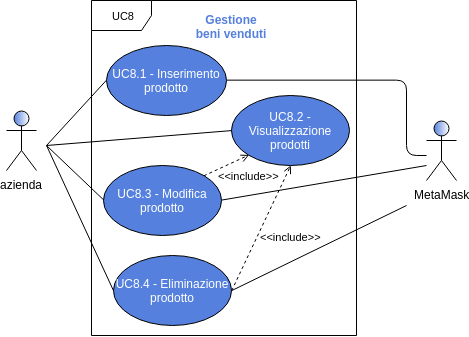
\includegraphics[width=10cm]{res/images/UC8-Generale.png}
	\centering
	\caption{Operazioni per la gestione dei beni venduti}
\end{figure}
\begin{itemize}
	\item \textbf{Attori Primari}: azienda;
	\item \textbf{Attori Secondari}: MetaMask\glo;
	\item \textbf{Descrizione}: le aziende hanno la possibilità di gestire i beni venduti sulla piattaforma;
	\item \textbf{Scenario principale}: l'azienda accede alla pagina per la gestione dei prodotti/servizi venduti e può:
	\begin{itemize}
		\item inserire un nuovo prodotto/servizio da vendere [UC8.1];
		\item visualizzare i propri prodotti attualmente in vendita [UC8.2];
		\item modificare un prodotto/servizio già presente nella piattaforma [UC8.3];
		\item rimuovere un prodotto/servizio presente [UC8.4]; 
	\end{itemize}
	\item \textbf{Precondizione}: il sistema ha identificato l'utente come azienda, l'azienda ha espresso la volontà di gestire i propri prodotti/servizi;
	\item \textbf{Postcondizione}: il sistema fornisce all'azienda le operazioni che possono essere svolte sui propri prodotti.	
\end{itemize}

\subsubsection{UC8.1 - Inserimento prodotto}
\begin{figure}[H]
	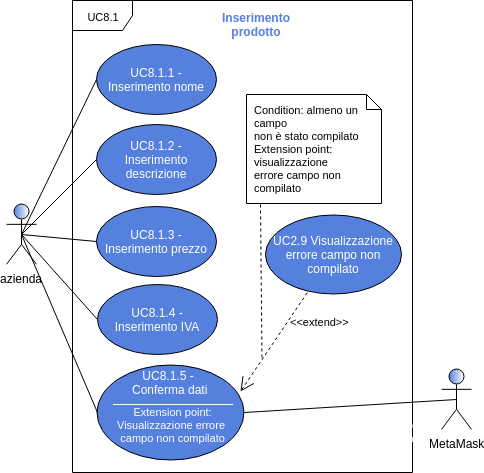
\includegraphics[width=10cm]{res/images/UC8-Inserimento.png}
	\centering
	\caption{Inserimento prodotto}
\end{figure}
\begin{itemize}
	\item \textbf{Attori Primari}: azienda;
	\item \textbf{Attori Secondari}: MetaMask\glo;
	\item \textbf{Descrizione}: le aziende possono inserire dei nuovi prodotti nella piattaforma;
	\item \textbf{Scenario principale}: l'azienda accede alla pagina per inserire un nuovo prodotto e deve:
	\begin{itemize}
		\item inserire il nome del prodotto/servizio [UC8.1.1];
		\item inserire la descrizione del prodotto/servizio [UC8.1.2];
		\item inserire il prezzo netto unitario del prodotto/servizio [UC8.1.3];
		\item inserire la quantità disponibile del prodotto/servizio [UC8.1.4];
		\item confermare i dati inseriti [UC8.1.5];
		\item inserire l'IVA del prodotto/servizio [UC8.1.6].
	\end{itemize}
	\item \textbf{Precondizione}: il sistema ha identificato l'utente come azienda, l'azienda ha espresso la volontà di inserire un nuovo prodotto/servizio;
	\item \textbf{Postcondizione}: l'azienda ha inserito correttamente i dati relativi al nuovo prodotto ed è riuscita ad inserire il nuovo prodotto/servizio sulla piattaforma.	
\end{itemize}
\subsubsection{UC8.1.1 - Inserimento nome}
\begin{itemize}
	\item \textbf{Attori Primari}: azienda;
	\item \textbf{Descrizione}: al fine di portare a termine il processo di inserimento di un nuovo prodotto l'utente deve inserire il nome del prodotto, campo ritenuto obbligatorio;
	\item \textbf{Scenario principale}: l'utente compila il campo relativo al nome del nuovo prodotto/servizio da inserire;
	\item \textbf{Precondizione}: il sistema ha reso disponibile il form per l'inserimento di un nuovo prodotto/servizio, in particolare è presente il campo per l'inserimento del nome;
	\item \textbf{Postcondizione}: l'utente ha compilato il campo relativo al nome del nuovo prodotto da inserire.
\end{itemize}
\subsubsection{UC8.1.2 - Inserimento descrizione}
\begin{itemize}
	\item \textbf{Attori Primari}: azienda;
	\item \textbf{Descrizione}: al fine di portare a termine il processo di inserimento di un nuovo prodotto l'utente deve inserire la descrizione del prodotto, campo ritenuto obbligatorio;
	\item \textbf{Scenario principale}: l'utente compila il campo relativo alla descrizione del nuovo prodotto/servizio da inserire;
	\item \textbf{Precondizione}: il sistema ha reso disponibile il form per l'inserimento di un nuovo prodotto/servizio, in particolare è presente il campo per l'inserimento della descrizione;
	\item \textbf{Postcondizione}: l'utente ha compilato il campo relativo alla descrizione del nuovo prodotto da inserire.
\end{itemize}
\subsubsection{UC8.1.3 - Inserimento prezzo netto}
\begin{itemize}
	\item \textbf{Attori Primari}: azienda;
	\item \textbf{Descrizione}: al fine di portare a termine il processo di inserimento di un nuovo prodotto l'utente deve inserire il prezzo netto unitario del prodotto, campo ritenuto obbligatorio;
	\item \textbf{Scenario principale}: l'utente compila il campo relativo al prezzo del nuovo prodotto/servizio da inserire;
	\item \textbf{Precondizione}: il sistema ha reso disponibile il form per l'inserimento di un nuovo prodotto/servizio, in particolare è presente il campo per l'inserimento del prezzo;
	\item \textbf{Postcondizione}: l'utente ha compilato il campo relativo al prezzo del nuovo prodotto da inserire.
\end{itemize}
\subsubsection{UC8.1.4 - Inserimento quantità}
\begin{itemize}
	\item \textbf{Attori Primari}: azienda;
	\item \textbf{Descrizione}: al fine di portare a termine il processo di inserimento di un nuovo prodotto l'utente deve inserire il numero di pezzi disponibili del prodotto, campo ritenuto obbligatorio;
	\item \textbf{Scenario principale}: l'utente compila il campo relativo al numero di pezzi del nuovo prodotto/servizio da inserire;
	\item \textbf{Precondizione}: il sistema ha reso disponibile il form per l'inserimento di un nuovo prodotto/servizio, in particolare è presente il campo per l'inserimento alla quantità di pezzi;
	\item \textbf{Postcondizione}: l'utente ha compilato il campo relativo alla quantità di pezzi del nuovo prodotto da inserire.
\end{itemize}
\subsubsection{UC8.1.5 - Conferma dati}
\begin{itemize}
	\item \textbf{Attori Primari}: azienda;
	\item \textbf{Attori Primari}: MetaMask\glo;
	\item \textbf{Descrizione}: al fine di portare a termine il processo di registrazione l'utente deve confermare i dati inseriti tramite l'approvazione della transazione, che verrà eseguita attraverso il plugin MetaMask\glo;
	\item \textbf{Scenario principale}: l'utente preme il pulsante di conferma dei dati inseriti e valida la transazione con MetaMask\glo;
	\item \textbf{Estensioni}:
	\begin{itemize}
		\item \textbf{UC2.9}: l'utente tenta di confermare i dati senza aver compilato tutti i campi richiesti;
	\end{itemize}
	\item \textbf{Precondizione}: il sistema ha reso disponibile il form per l'inserimento dei dati riguardanti il nuovo prodotto, l'utente ha compilato tutti i campi ed ha premuto il pulsante per la conferma.
	\item \textbf{Postcondizione}: il nuovo prodotto è stato inserito nella piattaforma e l'utente ottiene la conferma della riuscita dell'operazione.
\end{itemize}
\subsubsection{UC8.1.6 - Inserimento IVA}
\begin{itemize}
	\item \textbf{Attori Primari}: azienda;
	\item \textbf{Descrizione}: al fine di portare a termine il processo di inserimento di un nuovo prodotto l'utente deve inserire la percentuale di IVA;
	\item \textbf{Scenario principale}: l'utente compila il campo relativo all'IVA del nuovo prodotto/servizio da inserire;
	\item \textbf{Precondizione}: il sistema ha reso disponibile il form per l'inserimento di un nuovo prodotto/servizio, in particolare è presente il campo per l'inserimento dell'IVA;
	\item \textbf{Postcondizione}: l'utente ha compilato il campo relativo all'IVA del nuovo prodotto da inserire.
\end{itemize}
\subsubsection{UC8.2 - Visualizzazione prodotto}
\begin{figure}[h]
	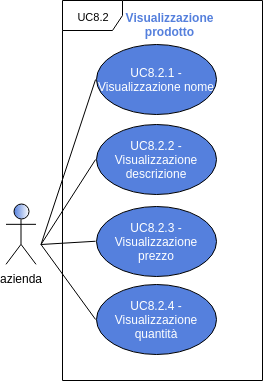
\includegraphics[width=6cm]{res/images/UC8-Visualizzazione.png}
	\centering
	\caption{Inserimento prodotto}
\end{figure}
\begin{itemize}
	\item \textbf{Attori Primari}: azienda;
	\item \textbf{Descrizione}: le aziende possono visualizzare i loro prodotti inseriti nella piattaforma;
	\item \textbf{Scenario principale}: l'azienda accede alla pagina per visualizzare i loro prodotti. Per ogni prodotto potrà: 
	\begin{itemize}
		\item visualizzare il nome [UC8.2.1];
		\item visualizzare la descrizione [UC8.2.2];
		\item visualizzare il prezzo [UC8.2.3];
		\item visualizzare la quantità [UC8.2.4];
	\end{itemize}
	\item \textbf{Precondizione}: il sistema ha identificato l'utente come azienda, l'azienda ha espresso la volontà di visualizzare i propri prodotti inseriti nella piattaforma;
	\item \textbf{Postcondizione}: l'azienda ha ottenuto la lista dei propri prodotti assieme alle operazioni eseguibili su di essi.	
\end{itemize}
\subsubsection{UC8.2.1 - Visualizzazione nome}
\begin{itemize}
	\item \textbf{Attori Primari}: azienda;
	\item \textbf{Descrizione}: l'azienda visualizza il nome del bene o del servizio;
	\item \textbf{Scenario principale}: l'utente visualizza le informazioni relative ai propri prodotti/servizi;
	\item \textbf{Precondizione}: l'utente ha espresso la volontà di visualizzare i propri prodotti/servizi;
	\item \textbf{Postcondizione}: l'utente può visualizzare il nome del prodotto.
\end{itemize}
\subsubsection{UC8.2.2 - Visualizzazione quantità}
\begin{itemize}
	\item \textbf{Attori Primari}: azienda;
	\item \textbf{Descrizione}: l'azienda visualizza la quantità rimanente del bene o del servizio;
	\item \textbf{Scenario principale}: l'utente visualizza le informazioni relative ai propri prodotti/servizi;
	\item \textbf{Precondizione}: l'utente ha espresso la volontà di visualizzare i propri prodotti/servizi;
	\item \textbf{Postcondizione}: l'utente può visualizzare la quantità rimanente di ciascuno dei prodotti.
\end{itemize}
\subsubsection{UC8.2.3 - Visualizzazione prezzo}
\begin{itemize}
	\item \textbf{Attori Primari}: azienda;
	\item \textbf{Descrizione}: l'azienda visualizza il prezzo del bene o del servizio;
	\item \textbf{Scenario principale}: l'utente visualizza le informazioni relative ai propri prodotti/servizi;
	\item \textbf{Precondizione}: l'utente ha espresso la volontà di visualizzare i propri prodotti/servizi;
	\item \textbf{Postcondizione}: l'utente può visualizzare il prezzo del prodotto.
\end{itemize}
\subsubsection{UC8.2.4 - Visualizzazione descrizione}
\begin{itemize}
	\item \textbf{Attori Primari}: azienda;
	\item \textbf{Descrizione}: l'azienda visualizza la descrizione del bene o del servizio;
	\item \textbf{Scenario principale}: l'utente visualizza le informazioni relative ai propri prodotti/servizi;
	\item \textbf{Precondizione}: l'utente ha espresso la volontà di visualizzare i propri prodotti/servizi;
	\item \textbf{Postcondizione}: l'utente può visualizzare la descrizione del prodotto.
\end{itemize}

\subsubsection{UC8.3 - Modifica prodotto}
\begin{figure}[H]
	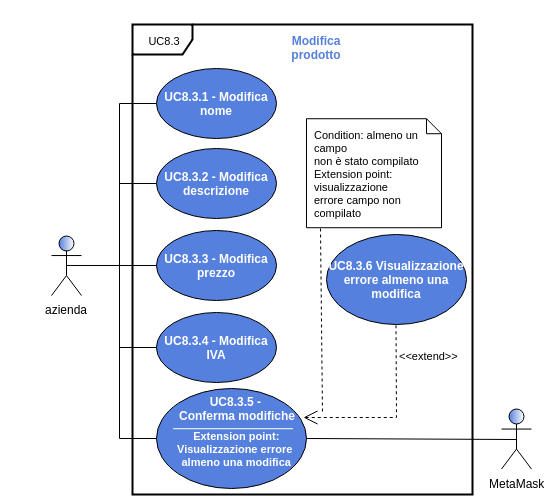
\includegraphics[width=10cm]{res/images/UC8-Modifica.png}
	\centering
	\caption{Inserimento prodotto}
\end{figure}
\begin{itemize}
	\item \textbf{Attori Primari}: azienda;
	\item \textbf{Attori Secondari}: MetaMask\glo;
	\item \textbf{Descrizione}: le aziende possono modificare i loro prodotti inseriti nella piattaforma;
	\item \textbf{Scenario principale}: l'azienda accede alla modifica di un prodotto attraverso l'apposito pulsante mostrato assieme alle informazioni riguardanti l'oggetto stesso[UC8.2]. Per ogni prodotto potrà: 
	\begin{itemize}
		\item modificarne il nome [UC8.3.1];
		\item modificarne la descrizione [UC8.3.2];
		\item modificarne il prezzo [UC8.3.3];
		\item modificarne la quantità [UC8.3.4];
	\end{itemize}
	Dunque dovrà confermare l'operazione attraverso l'utilizzo di MetaMask\glo.
	\item \textbf{Inclusione}:
	\begin{itemize}
		\item \textbf{UC8.2}: per poter modificare i prodotti l'azienda deve prima individuarli nella lista dei propri prodotti;
	\end{itemize}
	\item \textbf{Precondizione}: il sistema ha identificato l'utente come azienda, l'azienda ha espresso la volontà modificare un prodotto;
	\item \textbf{Postcondizione}: l'azienda ha modificato le caratteristiche del prodotto ed ha ottenuto un messaggio che conferma il successo dell'operazione.	
\end{itemize}

\subsubsection{UC8.3.1 - Modifica nome}
\begin{itemize}
	\item \textbf{Attori Primari}: azienda;
	\item \textbf{Descrizione}: l'azienda inserisce nell'apposito campo il nuovo nome del prodotto/servizio;
	\item \textbf{Scenario principale}: l'utente visualizza il vecchio nome con affianco un campo dati per inserire il nuovo nome, ed inserisce il nuovo valore;
	\item \textbf{Precondizione}: l'utente ha espresso la volontà di modificare i dati di un prodotto/servizio;
	\item \textbf{Postcondizione}: l'utente ha inserito il nuovo nome nel campo dedicato del form.
\end{itemize}

\subsubsection{UC8.3.2 - Modifica descrizione}
\begin{itemize}
	\item \textbf{Attori Primari}: azienda;
	\item \textbf{Descrizione}: l'azienda inserisce nell'apposito campo la nuova descrizione del prodotto/servizio;
	\item \textbf{Scenario principale}: l'utente visualizza la vecchia descrizione con affianco un campo dati per inserire la nuova descrizione, ed inserisce il nuovo valore;
	\item \textbf{Precondizione}: l'utente ha espresso la volontà di modificare i dati di un prodotto/servizio;
	\item \textbf{Postcondizione}: l'utente ha inserito la nuova descrizione nel campo dedicato del form.
\end{itemize}

\subsubsection{UC8.3.3 - Modifica prezzo}
\begin{itemize}
	\item \textbf{Attori Primari}: azienda;
	\item \textbf{Descrizione}: l'azienda inserisce nell'apposito campo il nuovo prezzo del prodotto/servizio;
	\item \textbf{Scenario principale}: l'utente visualizza il vecchio prezzo con affianco un campo dati per inserire il nuovo prezzo, ed inserisce il nuovo valore;
	\item \textbf{Precondizione}: l'utente ha espresso la volontà di modificare i dati di un prodotto/servizio;
	\item \textbf{Postcondizione}: l'utente ha inserito il nuovo prezzo nel campo dedicato del form.
\end{itemize}

\subsubsection{UC8.3.4 - Modifica quantità}
\begin{itemize}
	\item \textbf{Attori Primari}: azienda;
	\item \textbf{Descrizione}: l'azienda inserisce nell'apposito campo la nuova quantità del prodotto/servizio;
	\item \textbf{Scenario principale}: l'utente visualizza la vecchia quantità con affianco un campo dati per inserire la nuova quantità, ed inserisce il nuovo valore;
	\item \textbf{Precondizione}: l'utente ha espresso la volontà di modificare i dati di un prodotto/servizio;
	\item \textbf{Postcondizione}: l'utente ha inserito la nuova quantità nel campo dedicato del form.
\end{itemize}

\subsubsection{UC8.3.5 - Conferma modifiche}
\begin{itemize}
	\item \textbf{Attori Primari}: azienda;
	\item \textbf{Attori Primari}: MetaMask\glo;
	\item \textbf{Descrizione}: al fine di portare a termine il processo di modifica dei dati di un prodotto/servizio, l'utente deve confermare i dati inseriti tramite l'approvazione della transazione, che verrà eseguita attraverso il plugin MetaMask\glo;
	\item \textbf{Scenario principale}: l'utente preme il pulsante di conferma dei dati inseriti e valida l'operazione con MetaMask\glo;
	\item \textbf{Estensioni}:
	\begin{itemize}
		\item \textbf{UC8.3.6}: l'utente tenta di confermare i dati senza aver compilato almeno uno dei campi;
	\end{itemize}
	\item \textbf{Precondizione}: il sistema ha reso disponibile il form per la modifica dei dati riguardanti un prodotto. L'utente ha compilato almeno un campo ed ha premuto il pulsante per la conferma.
	\item \textbf{Postcondizione}: il prodotto è stato aggiornato con i nuovi dati e l'utente ottiene la conferma della riuscita dell'operazione.
\end{itemize}

\subsubsection{UC8.3.6 - Visualizzazione errore almeno una modifica}
\begin{itemize}
	\item \textbf{Attori Primari}: azienda;
	\item \textbf{Descrizione}:
	l'utente visualizza un messaggio di errore relativo al fatto nessuno dei campi per la modifica è stato compilato, e che quindi non è possibile attuare alcuna modifica;
	\item \textbf{Scenario principale}: l'utente tenta di confermare ed inviare le modifiche ai dati senza aver compilato almeno uno dei campi del form;
	\item \textbf{Precondizione}: il sistema permette all'utente di compilare il form per le modifiche. L'utente ha premuto il pulsante di conferma senza aver modificato almeno uno dei campi; 
	\item \textbf{Postcondizione}:
	l'utente è consapevole che per effettuare una modifica, almeno uno dei dati presenti deve essere stato modificato, compilando almeno uno dei campi del form.
\end{itemize}

\subsubsection{UC8.4 - Eliminazione prodotto}
\begin{itemize}
	\item \textbf{Attori Primari}: azienda;
	\item \textbf{Attori Primari}: MetaMask\glo;
	\item \textbf{Descrizione}:
	l'utente elimina uno dei propri prodotti/servizi presenti sulla piattaforma;
	\item \textbf{Scenario principale}: l'utente clicca sul pulsante di eliminazione prodotto, mostrato assieme alle informazioni riguardanti l'oggetto stesso [UC8.2]. Dunque dovrà confermare l'operazione attraverso l'utilizzo di MetaMask\glo;
	\item \textbf{Inclusione}:
	\begin{itemize}
		\item \textbf{UC8.2}: per poter eliminare i prodotti l'azienda deve prima individuarli nella lista dei propri prodotti;
	\end{itemize}
	\item \textbf{Precondizione}: il sistema ha identificato l'utente come azienda, l'azienda ha espresso la volontà eliminare un prodotto;
	\item \textbf{Postcondizione}: l'azienda ha eliminato il prodotto ed ha ottenuto un messaggio che conferma il successo dell'operazione.
\end{itemize}



\pagebreak
\subsubsection*{Operazioni governative}
Di seguito sono riportati tutti i casi d'uso che coinvolgono come attore primario il governo.

\begin{figure}[H]
	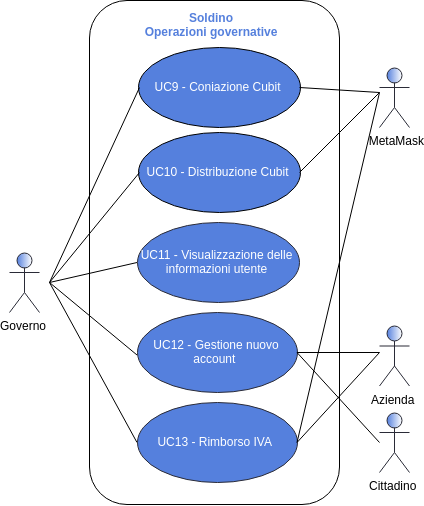
\includegraphics[width=8cm]{res/images/UseCaseGoverno.png}
	\centering
	\caption{Use cases che interessano il governo}
\end{figure}
\subsubsection{UC9 - Coniazione Cubit}
\begin{itemize}
	\item \textbf{Attori Primari}: governo;
	\item \textbf{Attori Secondari}: MetaMask\glo;
	\item \textbf{Descrizione}: viene coniata una quantità definita di Cubit\glo;
	
	\item \textbf{Scenario principale}: il governo ritiene necessario coniare ulteriori Cubit rispetto a quelli attualmente presenti sul mercato. Per fare ciò deve accedere alla pagina dedicata in cui, attraverso un form dovrà:
	 \begin{enumerate}[label=\alph*.]
		\item inserire la quantità $x$ di Cubit da coniare;
		\item confermare tale operazione attraverso l'utilizzo di MetaMask\glo.
	\end{enumerate}
	\item \textbf{Precondizione}: sia $x$ l'ammontare di Cubit che il governo 
	vuole coniare e $n$ l'ammontare di Cubit attualmente in circolo. L'utente 
	governativo è acceduto alla pagina per la coniazione ed ha compilato e 
	confermato il form;
	\item \textbf{Postcondizione}: i Cubit in circolo sono $x+n$.
\end{itemize}
\subsubsection{UC10 - Distribuzione Cubit}
%non capisco perchè la figura è prima del titolo sul PDF
\begin{figure}[h]
	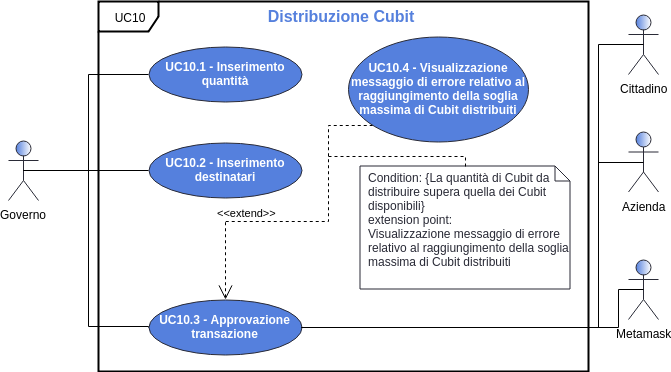
\includegraphics[width=13.5cm]{res/images/UC10Distribuzione.png} %da adattare in larghezza
	\centering
	\caption{UC10 - Distribuzione Cubit}
	
\end{figure}
\begin{itemize}
	\item \textbf{Attori Primari}: governo;
	\item \textbf{Attori Secondari}: MetaMask\glo, cittadino, azienda\glo;
	\item \textbf{Descrizione}: il governo trasferisce una somma di Cubit\glosp sull'account di uno o più  utenti, che siano essi cittadini o aziende;
	\item \textbf{Scenario principale}: il governo deve:
	 \begin{enumerate}[label=\alph*.]
		\item determinare l'ammontare di Cubit pro capite da trasferire [UC10.1];
		\item  selezionare la lista dei destinatari del trasferimento dalla lista degli utenti [UC10.2];
		\item confermare l'operazione [UC10.3].
	\end{enumerate}

	\item \textbf{Precondizione}: il governo accede alla pagina contenente il form per la distribuzione di Cubit agli utenti e compila il suddetto form;
	\item \textbf{Postcondizione}: tali utenti ricevono i Cubit da parte del governo.
\end{itemize}
\subsubsection{UC10.1 - Inserimento quantità}
\begin{itemize}
	\item \textbf{Attori Primari}: governo;
	\item \textbf{Descrizione}: il governo inserisce nell'apposito campo del form la quantità di Cubit\glosp da distribuire, ritenendo la quantità inserita come quantità da inviare ad ogni singolo utente;
	\item \textbf{Scenario principale}: il governo inserisce l'ammontare $x$ di 
	Cubit da inviare;
	\item \textbf{Precondizione}: il governo accede alla pagina contenente il form per la distribuzione di Cubit agli utenti e compila il campo relativo alla quantità;
	\item \textbf{Postcondizione}: il campo relativo all'ammontare di Cubit da 
	distribuire pro capite è stato compilato. 
\end{itemize}
\subsubsection{UC10.2 - Inserimento destinatari}
\begin{itemize}
	\item \textbf{Attori Primari}: governo;
	\item \textbf{Attori Secondari}: cittadino, azienda;
	\item \textbf{Descrizione}: il governo inserisce nell'apposito form la lista dei destinatari della quantità di Cubit\glosp precedentemente inserita;
	\item \textbf{Scenario principale}: il governo:
	\begin{enumerate}[label=\alph*.]
		\item visualizza delle liste contenenti i cittadini e le aziende registrate al sito [UC11.1 \& UC11.2], che sono accompagnati da una checkbox;
		\item l'utente può usare una barra di ricerca per individuare dei particolari utenti [UC16];
		\item l'utente governativo spunta le caselle relative agli utenti ai quali intende trasferire la quantità di Cubit precedentemente definita.
	\end{enumerate}
	\item \textbf{Inclusioni}:
	\begin{itemize}
		\item \textbf{UC11}: per poter selezionare i destinatari, l'utente deve prima visualizzare la lista degli utenti registrati alla piattaforma, eventualmente filtrando i risultati.
	\end{itemize}
	\item \textbf{Precondizione}: il governo si trova nella pagina atta alla distribuzione dei Cubit;
	\item \textbf{Postcondizione}: il governo ha selezionato uno o più destinatari dalle liste degli utenti, e può procedere con l'approvazione della transazione.
\end{itemize}
\subsubsection{UC10.3 - Approvazione transazione}
\begin{itemize}
	\item \textbf{Attori Primari}: governo;
	\item \textbf{Attori Secondari}: MetaMask\glo, cittadino, azienda\glo;
	\item \textbf{Descrizione}: il governo decide se approvare o rifiutare la transazione;
	\item \textbf{Scenario principale}: il governo ha specificato la somma 
	$x$ di Cubit\glosp da distribuire ad ognuno degli $y$ destinatari;
	\item \textbf{Estensioni}:
	\begin{itemize}
		\item \textbf{UC10.4}: verrà mostrato un messaggio di errore nel caso 
		l'ammontare totale $x\cdot y$ superi la quantità di \textit{Cubit} disponibili 
		alla distribuzione.
	\end{itemize}
	\item \textbf{Precondizione}: è necessario aver selezionato una lista di destinatari ed una quantità da distribuire ad ogni singolo utente;
	\item \textbf{Postcondizione}: ogni utente riceverà nel proprio wallet\glosp la quantità di Cubit trasferita dal governo.
\end{itemize}
\subsubsection{UC10.4 - Visualizzazione messaggio di errore relativo al raggiungimento della soglia massima di Cubit distribuiti}
\begin{itemize}
	\item \textbf{Attori Primari}: governo;
	\item \textbf{Descrizione}: il governo riceve un messaggio di errore relativo al fatto che ha selezionato una quantità di Cubit\glosp superiore a quella disponibile alla distribuzione;
	\item \textbf{Scenario principale}: il governo clicca sull'apposito pulsante per confermare la transazione di distribuzione, ma non ha sufficienti fondi per completare tale operazione;
	\item \textbf{Precondizione}: il governo deve aver inserito una quantità di Cubit superiore a quella disponibile e cerca di effettuare la transazione;
	\item \textbf{Postcondizione}: viene visualizzato un messaggio d'errore per informare l'utente del fatto che attualmente non dispone dei fondi necessari per effettuare l'operazione di distribuzione.
	
\end{itemize} 

 \subsubsection{UC11 - Visualizzazione delle informazioni utente}
 \begin{figure}[h]
 	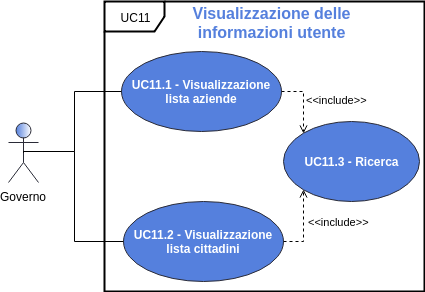
\includegraphics[width=7cm]{res/images/UC11-Generale.png}
 	\centering
 	\caption{UC11 - Visualizzazione delle informazioni utente}
 	
 \end{figure}
 \begin{itemize}
 	\item \textbf{Attori Primari}: governo;
 	\item \textbf{Descrizione}: il governo può accedere alle informazioni riguardanti:
 	\begin{itemize}
 		\item le aziende registrate alla piattaforma;
 		\item i cittadini registrati alla piattaforma;

 	\end{itemize}
 	\item \textbf{Scenario principale}: il governo accede alle informazioni riguardanti gli utenti della piattaforma ed alle eventuali relative operazioni disponibili;

 	\item \textbf{Precondizione}: il sistema riconosce che l'utente è autenticato con privilegi governativi e mostra le pagine utili alla ricerca di informazioni sugli utenti;
 	
 	\item \textbf{Postcondizione}: il governo ottiene dal sistema le liste degli utenti con le eventuali operazioni disponibili.
 \end{itemize}

\subsubsection{UC11.1 - Visualizzazione lista aziende registrate}
\begin{figure}[H]
	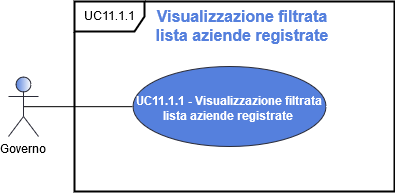
\includegraphics[width=7cm]{res/images/UC11-VisualizzazioneFiltrata.png}
	\centering
	\caption{UC11 - Visualizzazione lista aziende registrate}
	
\end{figure}
 \begin{itemize}
	\item \textbf{Attori Primari}: governo;
	\item \textbf{Descrizione}: il governo visualizza la lista delle aziende registrate alla piattaforma. Per ogni azienda sono rese disponibili le seguenti informazioni:
	\begin{itemize}
		\item chiave\glosp Ethereum\glo;
		\item nome (ragione sociale);
		\item partita IVA;
		\item indirizzo di residenza (sede dell'azienda);
		\item lo stato di "abilitato" o "disabilitato";
		\item indirizzo email;
		\item lo stato del pagamento del saldo IVA, ovvero può controllare se l'azienda risulta:
		\begin{itemize}
			\item \textbf{insolvente}: non ha ancora provveduto alla liquidazione IVA di almeno uno dei trimestri precedenti entro i termini fissati;
			\item \textbf{in fase di pagamento}: l'azienda deve ancora effettuare il versamento IVA riguardante l'ultimo trimestre, ed il termine del pagamento non è ancora scaduto. Nei trimestri antecedenti la situazione risulta "regolare";
			\item \textbf{in dilazione}: in caso l'azienda abbia richiesto il pagamento dilazionato del saldo IVA a debito ed il termine della dilazione non è ancora scaduto;
			\item \textbf{regolare}: l'azienda ha provveduto al pagamento del saldo IVA a debito del trimestre precedente oppure ha ricevuto il rimborso nel caso in cui sia risultata "In attesa di rimborso" nel trimestre precedente;
			\item \textbf{in attesa di rimborso}: nel trimestre precedente il saldo IVA è risultato a credito, e non è ancora stato effettuato il rimborso da parte del governo;
		\end{itemize}
	L'azienda può ricadere in uno solo tra i casi sopra descritti. Lo stato di insolvenza di un trimestre precedente ha la predominanza sugli stati dei trimestri successivi ad esso;
		\item l'importo del saldo IVA;
	\end{itemize}
	
	\item \textbf{Scenario principale}: il governo richiede la lista delle aziende registrate;
	\item \textbf{Inclusioni}:
	\begin{itemize}
		\item \textbf{UC16}: l'utente può filtrare i risultati visualizzati inserendo una parola chiave;
	\end{itemize}
	\item \textbf{Precondizione}: il sistema riconosce che l'utente è autenticato con privilegi governativi ed ha richiesto di ottenere la lista di tutte aziende;
	\item \textbf{Postcondizione}: il governo ottiene dal sistema la lista delle aziende registrate, con associate le operazioni che può effettuare su di esse.
\end{itemize}

\subsubsection{UC11.1.1 - Visualizzazione filtrata lista aziende registrate}
\begin{itemize}
	\item \textbf{Attori Primari}: governo;
	\item \textbf{Descrizione}: il governo visualizza la lista delle aziende registrate alla piattaforma, filtrate secondo il valore del campo \texttt{stato del pagamento del saldo IVA}. I possibili valori per filtrare i risultati per tale campo sono i seguenti:
	\begin{itemize}
		\item insolvente;
		\item in fase di pagamento;
		\item in dilazione
		\item regolare;
		\item in attesa di rimborso;
	\end{itemize}
	
	\item \textbf{Scenario principale}: il governo filtra le aziende visualizzate secondo il valore del campo \texttt{stato del pagamento del saldo IVA}. Seleziona tale valore servendosi dell'apposito menù a tendina;
	\item \textbf{Precondizione}: l'utente governativo ha eseguito l'accesso alla pagina dedicata alla visualizzazione delle aziende registrate, ed ha selezionato un'opzione per filtrare le aziende;
	\item \textbf{Postcondizione}: il governo ottiene dal sistema la lista delle aziende registrate, filtrate a seconda del valore del campo \texttt{stato del pagamento del saldo IVA} selezionato.
\end{itemize}


\subsubsection{UC11.2 - Visualizzazione lista cittadini}
\begin{itemize}
	\item \textbf{Attori Primari}: governo;
	\item \textbf{Descrizione}: il governo ottiene la lista dei cittadini. Per ognuno di essi può visualizzare:
	\begin{itemize}
		\item la chiave\glosp Ethereum\glo;
		\item il nome;
		\item il cognome;
		\item l'indirizzo di residenza;
		\item indirizzo email;
	\end{itemize}
	\item \textbf{Scenario principale}: il governo richiede la lista dei cittadini. Per ognuno di essi visualizza le rispettive informazioni;
	\item \textbf{Inclusioni}:
	\begin{itemize}
		\item \textbf{UC16}: l'utente può filtrare i risultati visualizzati inserendo una parola chiave;
	\end{itemize}
	\item \textbf{Precondizione}: il sistema riconosce che l'utente è autenticato con privilegi governativi ed ha richiesto di ottenere la lista di tutti i cittadini;
	\item \textbf{Postcondizione}: il governo ottiene dal sistema la lista dei cittadini, con associate le operazioni che può effettuare su di essi.
\end{itemize}



\subsubsection{UC12 - Validazione nuovo account registrato}
\begin{figure}[h]
	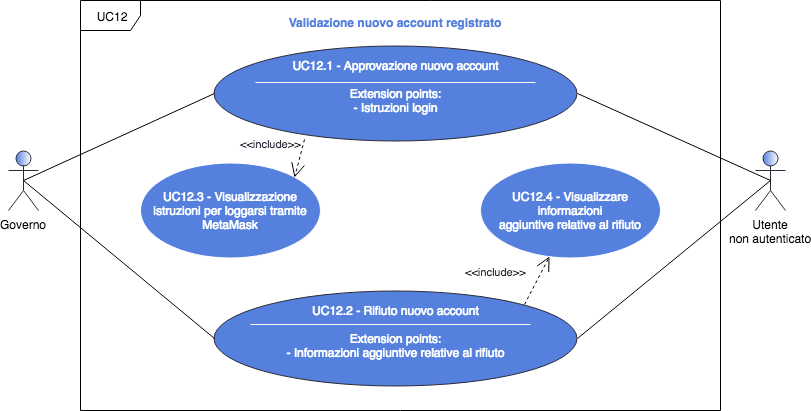
\includegraphics[width=15.5cm]{res/images/UC12Validazione.png} %da adattare in larghezza
	\centering
	\caption{UC12 - Validazione nuovo account registrato}
	
\end{figure}
\begin{itemize}
	\item \textbf{Attori Primari}:
	governo;
	\item \textbf{Attori Secondari}:
	utente non autenticato;
	\item \textbf{Descrizione}: l'account utente può venire rigettato o approvato dal governo;
	\item \textbf{Scenario principale}: l'utente si è registrato al sistema ma è ancora in attesa di una risposta da parte del governo in merito alla validazione del proprio account. Il flusso degli eventi è il seguente:
	\begin{enumerate}[label=\alph*.]
		\item il governo ottiene la lista delle aziende in lista di attesa [UC11.3] o dei cittadini in lista di attesa [UC11.4];
		\item il governo approva [UC12.1] o rifiuta [UC12.2] la richiesta di iscrizione;
	\end{enumerate}
	\item \textbf{Precondizione}: l'utente è in coda di attesa per la validazione dell'account;
	\item \textbf{Postcondizione}: l'account utente viene approvato o rigettato. 
\end{itemize}
\subsubsection{UC12.1 - Approvazione nuovo account}
\begin{itemize}
	\item \textbf{Attori Primari}:
	governo;
	\item \textbf{Attori Secondari}:
	utente non autenticato;
	\item \textbf{Descrizione}: l'account utente viene approvato;
	\item \textbf{Scenario principale}: in seguito alla registrazione, il governo riconosce validi i dati immessi dall'utente;
	\item \textbf{Inclusioni}:
	\begin{itemize}
		\item \textbf{UC12.3}: in seguito all'approvazione dell'account, l'utente visualizza una breve e concisa guida su come loggarsi al sito;
	\end{itemize}
	\item \textbf{Precondizione}: l'utente ha portato a termine la richiesta di registrazione ed è ancora in attesa di verifica;
	\item \textbf{Postcondizione}: l'utente è stato verificato e può visualizzare il modo corretto per eseguire il login alla piattaforma.
	
\end{itemize}
\subsubsection{UC12.2 - Rifiuto nuovo account}
\begin{itemize}
	\item \textbf{Attori Primari}:
	governo;
	\item \textbf{Attori Secondari}:
	utente non autenticato;
	\item \textbf{Descrizione}: l'account utente viene rifiutato;
	\item \textbf{Scenario principale}: in seguito alla registrazione, il governo riconosce non validi i dati immessi dall'utente;
	\item \textbf{Inclusioni}:
	\begin{itemize}
		\item \textbf{UC12.4}: in seguito al rigetto  dell'account, l'utente visualizza dettagli aggiuntivi del perchè non è stato accettato;
	\end{itemize}
	\item \textbf{Precondizione}: l'utente ha portato a termine la richiesta di registrazione ed è ancora in attesa di verifica;
	\item \textbf{Postcondizione}: l'utente risulta rifiutato e riceve le informazioni relative a tale rifiuto.
	
\end{itemize}
\subsubsection{UC12.3 - Visualizzazione istruzioni per loggarsi tramite MetaMask\glosp}
\begin{itemize}
	\item \textbf{Attori Primari}:
	governo;
	\item \textbf{Attori Secondari}:
	utente non autenticato;
	\item \textbf{Descrizione}: l'utente, durante il primo tentativo di accesso alla piattaforma dopo l'approvazione dell'account, visualizza una guida contenente le istruzioni per procedere al login tramite MetaMask\glo;
	\item \textbf{Scenario principale}: in seguito all'approvazione dell'account, l'utente cerca di effettuare il suo primo login, e gli vengono fornite tutte le istruzioni necessarie;
	\item \textbf{Precondizione}: l'utente è stato verificato e tenta di eseguire per la prima volta il login;
	\item \textbf{Postcondizione}: l'utente possiede le conoscenze necessarie al fine di conseguire un login corretto e sicuro tramite il plugin MetaMask\glo.
\end{itemize}
\subsubsection{UC12.4 - Visualizzazione informazioni aggiuntive in merito al rigetto dell'account}
\begin{itemize}
	\item \textbf{Attori Primari}:
	governo;
	\item \textbf{Attori Secondari}:
	utente non autenticato;
	\item \textbf{Descrizione}: l'utente visualizza le informazioni aggiuntive relative al rigetto del proprio account;
	\item \textbf{Scenario principale}: in seguito al rifiuto dell'account, l'utente riceve le informazioni relative a tale rigetto da parte del governo;
	\item \textbf{Precondizione}: l'utente non ha idea del perchè non è stato accettato;
	\item \textbf{Postcondizione}: l'utente riconosce di aver inserito dati falsi o contenenti errori, pertanto dovrà riprovare la registrazione.
\end{itemize} 
\subsubsection{UC13 - Rimborso IVA}
\begin{itemize}
	\item \textbf{Attori Primari}:
	governo;
	\item \textbf{Attori Secondari}:
	azienda, MetaMask\glo;
	\item \textbf{Descrizione}: il governo rimborsa l'IVA ad un'azienda che risulta in stato di credito al momento del saldo trimestrale;
	\item \textbf{Scenario principale}: dopo aver visualizzato lo stato dell'IVA di un'azienda [UC11.2.1] il governo decide di effettuare il rimborso cliccando sul pulsante dedicato. Dovrà confermare la transazione attraverso il plugin MetaMask\glo;
	\item \textbf{Estensioni}: 
	\begin{itemize}
		\item \textbf{UC7.5}: l'utente tenta il pagamento ma l'esito non va a buon fine. La causa del fallimento dell'operazione è gestito dal plugin stesso;
	\end{itemize}
	\item \textbf{Inclusioni}: 
	\begin{itemize}
		\item \textbf{UC11.2}: l'utente per poter accedere al pulsante per il rimborso dell'azienda deve visualizzare la lista delle aziende verificate;
	\end{itemize}
	\item \textbf{Precondizione}: il sistema ha mostrato la lista delle aziende già verificate, con il relativo stato dell'IVA. L'utente ha premuto il pulsante per il rimborso e confermato l'operazione;
	\item \textbf{Postcondizione}: il sistema avvisa l'utente che l'operazione è avvenuta con successo. Il rimborso è stato versato all'azienda.
\end{itemize} 

\subsubsection*{Operazioni di gestione degli ordini e delle fatture}
Di seguito sono riportate tutti i casi d'uso che coinvolgono la gestione degli ordine e delle fatture.

\begin{figure}[H]
	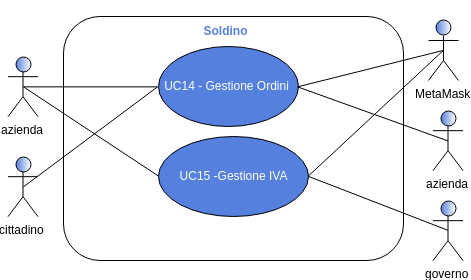
\includegraphics[width=8cm]{res/images/UseCaseFinali.png}
	\centering
	\caption{Use Cases riguardanti la gestione degli ordini e delle fatture}
\end{figure}
\subsubsection{UC14 - Gestione ordini}
\begin{figure}[h]
	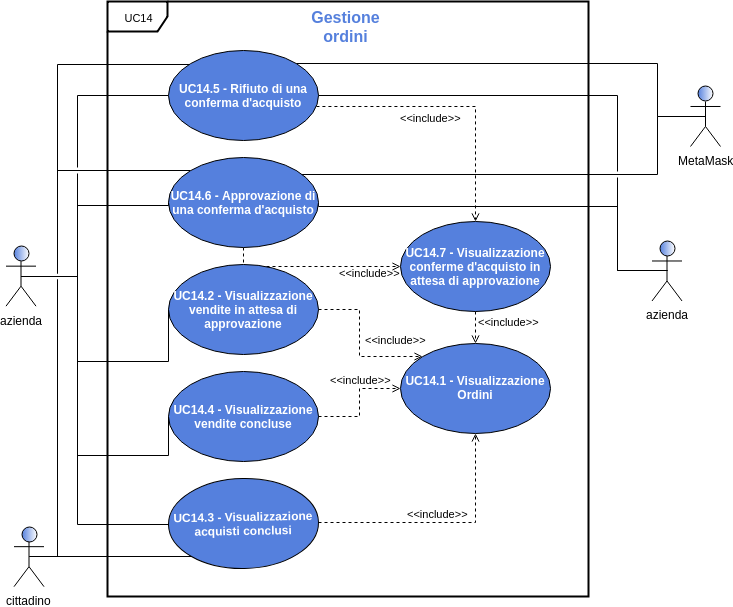
\includegraphics[width=10cm]{res/images/UC14-GestioneOrdini.png}
	\centering
	\caption{Gestione degli ordini}
\end{figure}
\begin{itemize}
	\item \textbf{Attori Primari}: azienda, cittadino;
	\item \textbf{Descrizione}: agli utenti sono messe a disposizione diverse operazione per visualizzare e gestire gli ordini;
	\item \textbf{Scenario principale}: l'utente visualizza e svolge alcune operazioni per gestire gli ordini dei quali ne è partecipe;
	\item \textbf{Precondizione}: il sistema ha riconosciuto l'utente autenticato come azienda o cittadino e mette a disposizione tutte le pagine necessarie alla visualizzazione e gestione degli ordini;
	\item \textbf{Postcondizione}: l'utente ha visualizzato e/o gestito i propri ordini.
\end{itemize} 
\subsubsection{UC14.1 - Visualizzazione ordini}
\begin{itemize}
	\item \textbf{Attori Primari}: azienda, cittadino;
	\item \textbf{Descrizione}: alle aziende ed ai cittadini sono messe a disposizione diverse operazione per visualizzare e gestire gli ordini all'interno della piattaforma. \`E reso possibile avere un elenco dettagliato di tutti gli ordini, in particolare per ognuno di essi è presente la:
	\begin{itemize}
		\item visualizzazione della data dell'ordine;
		\item visualizzazione del numero dell'ordine;
		\item visualizzazione dei prodotti inclusi nell'ordine [UC5];
		\item visualizzazione totale IVA;
		\item visualizzazione prezzo lordo\glo;
	\end{itemize}
	\item \textbf{Scenario principale}: l'utente visualizza degli ordini per poi poterli gestire;
	\item \textbf{Inclusioni}:
	\begin{itemize}
		\item \textbf{UC5}: visualizzazione dei beni;
	\end{itemize}
	\item \textbf{Precondizione}: il sistema ha riconosciuto l'utente autenticato come azienda o cittadino e mette a disposizione tutte le pagine necessarie alla visualizzazione e gestione degli ordini;
	\item \textbf{Postcondizione}: l'utente ha visualizzato e/o gestito i propri ordini.
\end{itemize} 

\subsubsection{UC14.2 - Visualizzazione vendite in attesa di approvazione}
\begin{itemize}
	\item \textbf{Attori Primari}: azienda;
	\item \textbf{Descrizione}: all'azienda è messa a disposizione la possibilità di visualizzare le vendite effettuate ad altre aziende, che sono in attesa di approvazione;
	\item \textbf{Scenario principale}: l'utente visualizza le vendite in attesa di approvazione tramite una vista dettagliata che include: 
		\begin{itemize}
		\item visualizzazione di tutte le informazioni dell'ordine [UC14.1];
		\item visualizzazione della data ultima per l'approvazione;
		\item visualizzazione nome azienda-cliente;
		\item visualizzazione partita IVA dell'azienda-cliente;
		\end{itemize}
		\item \textbf{Inclusioni}:
	\begin{itemize}
		\item \textbf{UC14.1}: Visualizzazione degli ordini;
	\end{itemize}
	\item \textbf{Precondizione}: il sistema ha riconosciuto l'utente autenticato come azienda visita la pagina per la visualizzazione delle vendite verso le aziende-clienti che sono ancora in attesa di approvazione;
	\item \textbf{Postcondizione}: l'utente ha visualizzato le proprie vendite in attesa di approvazione.
\end{itemize} 

\subsubsection{UC14.3 - Visualizzazione acquisti conclusi}
\begin{itemize}
	\item \textbf{Attori Primari}: cittadino, azienda;
	\item \textbf{Descrizione}: l'utente può visualizzare la lista degli acquisti conclusi;
	\item \textbf{Scenario principale}: l'utente visualizza la lista degli acquisti conclusi, che hanno un campo aggiuntivo, ovvero la data di conferma dell'ordine;
	\item \textbf{Inclusioni}:
	\begin{itemize}
		\item \textbf{UC14.1}: Visualizzazione degli ordini;
	\end{itemize}
	\item \textbf{Precondizione}: il sistema ha riconosciuto l'utente autenticato come azienda o cittadino e questo ha espresso la volontà di visualizzare la lista degli acquisti conclusi;
	\item \textbf{Postcondizione}: l'utente visualizza tale lista.
\end{itemize}

\subsubsection{UC14.4 - Visualizzazione vendite concluse}
\begin{itemize}
	\item \textbf{Attori Primari}: azienda;
	\item \textbf{Descrizione}: l'utente può visualizzare la lista delle proprie vendite ritenute concluse;
	\item \textbf{Scenario principale}: l'utente visualizza la lista delle vendite concluse, che hanno un campo aggiuntivo, ovvero la data di conferma dell'ordine da parte dell'azienda-cliente;
	\item \textbf{Inclusioni}:
	\begin{itemize}
		\item \textbf{UC14.1}: Visualizzazione degli ordini;
	\end{itemize}
	\item \textbf{Precondizione}: il sistema ha riconosciuto l'utente autenticato come azienda e questo ha espresso la volontà di visualizzare la lista delle vendite concluse;
	\item \textbf{Postcondizione}: l'utente visualizza tale lista.
\end{itemize}


\subsubsection{UC14.5 - Rifiuto di una conferma d'acquisto}
\begin{itemize}
	\item \textbf{Attori Primari}: azienda;
	\item \textbf{Attori Secondari}: MetaMask\glo, azienda;
	\item \textbf{Descrizione}: l'azienda può rifiutare una conferma d'acquisto\glo. Per effettuare l'operazione verrà utilizzato MetaMask\glo;
	\item \textbf{Scenario principale}: l'utente visualizza una conferma d'acquisto che necessitano di approvazione e decide di rifiutarla;
	\item \textbf{Inclusioni}: 
	\begin{itemize}
		\item \textbf{UC14.7}: visualizzazione delle conferme d'acquisto relative agli acquisti in attesa di approvazione;
	\end{itemize}
	\item \textbf{Precondizione}: il sistema ha riconosciuto l'utente autenticato come azienda ed ha mostrato la lista delle proposte d'acquisto che necessitano di conferma;
	\item \textbf{Postcondizione}: l'azienda ha rifiutato la proposta d'acquisto. La proposta non sarà più presente nella lista di attesa per la conferma. Il sistema ritorna l'ammontare trattenuto per l'ordine all'azienda-cliente.
\end{itemize}
\subsubsection{UC14.6 - Approvazione di una conferma di acquisto}
\begin{itemize}
	\item \textbf{Attori Primari}: azienda;
	\item \textbf{Attori Secondari}: MetaMask\glo, azienda;
	\item \textbf{Descrizione}: l'azienda accetta la proposta d'acquisto ricevuta;
	\item \textbf{Scenario principale}: l'azienda decide di approvare una proposta d'acquisto da parte di un acquirente. L'utente acquirente ha la possibilità di effettuare il versamento all'azienda-venditrice;
	\item \textbf{Scenario alternativo}: l'azienda non ha né confermato né approvato la conferma d'acquisto entro la data ultima per l'approvazione;
		\item \textbf{Inclusioni}: 
	\begin{itemize}
		\item \textbf{UC14.7}:  visualizzazione delle conferme d'acquisto relative agli acquisti in attesa di approvazione;
	\end{itemize}
	\item \textbf{Precondizione}: 
	\begin{enumerate}[label=\alph*.]
		\item il sistema ha riconosciuto l'utente autenticato come azienda, e questo ha espresso la volontà di approvare una richiesta d'acquisto;
		\item è stata superata la data ultima per l'approvazione della conferma d'ordine\glo;
	\end{enumerate}
	\item \textbf{Postcondizione}: il suddetto ordine risulta approvato dall'azienda.
\end{itemize}


\subsubsection{UC14.7 - Visualizzazione conferme d'acquisto in attesa di approvazione}
\begin{itemize}
	\item \textbf{Attori Primari}: azienda;
	\item \textbf{Descrizione}: l'azienda può visualizzare delle proposte d'acquisto che necessitano di conferma. Esse sono relative agli acquisti che ha effettuato ma non ancora confermato;
	\item \textbf{Scenario principale}: l'utente visualizza la lista delle proposte d'acquisto che necessitano di conferma. Per ognuna di esse ha a possibilità di confermare la proposta [UC14.6] o di rifiutarla [UC14.5];
	\item \textbf{Inclusioni}:
	\begin{itemize}
		\item \textbf{UC14.1}: Visualizzazione degli ordini;
	\end{itemize}
	\item \textbf{Precondizione}: il sistema ha riconosciuto l'utente autenticato come azienda e questo ha espresso la volontà di visualizzare la lista delle proposte d'acquisto che necessitano di conferma;
	\item \textbf{Postcondizione}: l'azienda visualizza tale lista.
\end{itemize}






\subsubsection{UC15 - Gestione transazioni ed IVA}
\begin{figure}[H]
	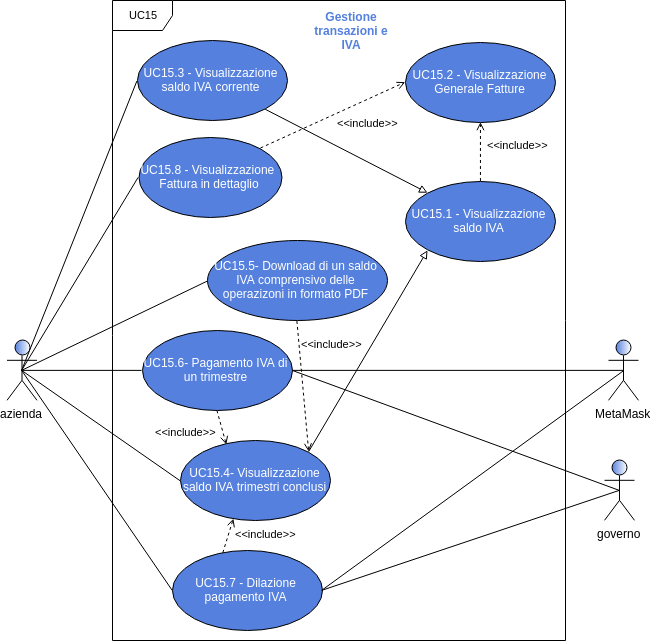
\includegraphics[width=8cm]{res/images/UC15-Generale.png}
	\centering
	\caption{UC15 - Operazioni riguardanti la gestione dell'IVA}
\end{figure}
\begin{itemize}
	\item \textbf{Attori Primari}: azienda;
	\item \textbf{Descrizione}: alle aziende sono messe a disposizione diverse operazioni per gestire le transazioni e l'IVA:
	\begin{itemize}
		\item può visulizzare i saldi IVA di un periodo, comprendendo la visualizzazione di tutte le transazioni, rappresentate dalla rispettiva fattura, e del saldo finale [15.3 \& 15.4];
		\item per ogni fattura è disponibile la visualizzazione dettagliata [15.8];
		\item può scaricare le informazioni riguardanti un trimestre come sopra descritto sotto forma di documento PDF [15.5]; 
		\item in caso il saldo di un semestre risulti negativo (situazione di debito), l'azienda può procedere ad effettuare il versamento al governo [15.6] o può dilazionarlo\glosp [15.7];
	\end{itemize}
	\item \textbf{Scenario principale}: l'utente visualizza e svolge alcune operazioni per gestire l'IVA, gli ordini e le fatture;
	\item \textbf{Precondizione}: il sistema ha riconosciuto l'utente autenticato come azienda, e mette a disposizione tutte le pagine necessarie alla visualizzazione e gestione delle fatture e dell'IVA;
	\item \textbf{Postcondizione}: l'azienda ha visualizzato e/o svolto delle operazioni riguardanti fatture ed IVA.
\end{itemize} 
\subsubsection{UC15.1 - Visualizzazione saldo IVA}
\begin{itemize}
	\item \textbf{Attori Primari}: azienda;
	\item \textbf{Descrizione}: l'azienda può visualizzare un saldo parziale relativo ad un trimestre IVA. In particolare può visualizzare il saldo:
	\begin{itemize}
		\item del trimestre corrente [15.3];
		\item di un trimestre concluso [15.4];
	\end{itemize}
	\item \textbf{Scenario principale}: l'utente visualizza il saldo parziale relativo ad un trimestre. In particolare:
	\begin{enumerate}[label=\alph*.]
		\item seleziona da un menù a tendina uno dei semestri disponibili;
		\item di questo semestre scelto viene visualizzata la relativa lista delle fatture; 
	\end{enumerate}
	\item \textbf{Inclusioni}: 
	\begin{itemize}
		\item \textbf{UC15.2}: visualizzazione generale delle fatture, ovvero il mostrare la lista delle fatture nel saldo;
	\end{itemize}
	\item \textbf{Specializzazioni}: 
	\begin{itemize}
		\item \textbf{UC15.3}: visualizzazione saldo IVA corrente;
		\item \textbf{UC15.4}:  visualizzazione saldo IVA di un trimestre concluso;
	\end{itemize}
	\item \textbf{Precondizione}: il sistema ha riconosciuto l'utente autenticato come azienda, e mette a disposizione le pagine per visualizzazione dei saldi dei semestri IVA;
	\item \textbf{Postcondizione}: l'azienda ha visualizzato il saldo IVA parziale riguardante il trimestre scelto ed è a conoscenza dalla situazione di debito o credito verso il governo.
\end{itemize} 
\subsubsection{UC15.2 - Visualizzazione generale fattura}
\begin{itemize}
	\item \textbf{Attori Primari}: azienda;
	\item \textbf{Descrizione}: per ogni fattura l'utente può visualizzare i seguenti campi:
	\begin{itemize}
		\item numero identificativo;
		\item data;
		\item nome dell'azienda venditrice/cliente;
		\item partita IVA dell'azienda venditrice/cliente;
		\item importo totale dell'ordine;
		\item IVA a credito/debito derivante dalla transazione;
	\end{itemize}
	\item \textbf{Scenario principale}: l'utente visualizza una fattura, riguardante i propri  acquisti o le vendite
	\item \textbf{Precondizione}: l'azienda sta visualizzando una pagina che richiede la visualizzazione dei dati generali di una fattura;
	\item \textbf{Postcondizione}: l'azienda ha visualizzato i dati relativi alla fattura.
\end{itemize}


\subsubsection{UC15.3 - Visualizzazione saldo IVA corrente}
\begin{itemize}
	\item \textbf{Attori Primari}: azienda;
	\item \textbf{Descrizione}: l'azienda può visualizzare il saldo parziale relativo al trimestre corrente, non ancora concluso. Non sono previste particolari operazioni per questa visualizzazione;
	\item \textbf{Scenario principale}: l'utente visualizza il saldo parziale relativo al trimestre corrente;
	\item \textbf{Precondizione}: l'utente ha selezionato la visualizzazione del saldo relativo al trimestre corrente;
	\item \textbf{Postcondizione}: l'azienda ha visualizzato il saldo IVA parziale riguardante il trimestre corrente ed è a conoscenza dall'attuale parziale situazione di debito o credito verso il governo.
\end{itemize} 

\subsubsection{UC15.4 - Visualizzazione saldo IVA trimestri conclusi}
\begin{itemize}
	\item \textbf{Attori Primari}: azienda;
	\item \textbf{Descrizione}: l'azienda può visualizzare la lista delle operazioni relative ad un trimestre IVA già concluso. Può inoltre leggerne lo stato, ovvero sapere se i pagamenti a debito o credito con il governo sono stati saldati oppure no. In caso di stato di debito relativo ad un trimestre, viene resa disponibile la data ultima per il versamento IVA, la possibilità di effettuare il pagamento, e quella di dilazionarlo;
	\item \textbf{Scenario principale}: l'utente visualizza la lista delle operazioni riguardanti  un saldo IVA relativo ad un trimestre concluso. Per ognuno di essi ottiene l'informazione sullo stato del pagamento dell'IVA, assieme alle operazioni che possono essere effettuate su di esso;
	\item \textbf{Precondizione}: l'utente ha selezionato la visualizzazione del saldo relativo ad un semestre concluso;
	\item \textbf{Postcondizione}: l'azienda ha visualizzato il saldo IVA riguardante un trimestre concluso, assieme alle possibili operazioni da effettuare.
\end{itemize} 

\subsubsection{UC15.5 - Download di un saldo IVA comprensivo delle operazioni in formato PDF}
\begin{itemize}
	\item \textbf{Attori Primari}: azienda;
	\item \textbf{Descrizione}: alle aziende è offerta la possibilità di scaricare le operazioni riguardanti un saldo trimestrale IVA nel formato PDF;
	\item \textbf{Scenario principale}: l'utente, dopo aver individuato il saldo desiderato, scarica, in formato PDF, l'elenco delle operazioni riguardanti il periodo trimestrale IVA selezionato;
	\item \textbf{Inclusioni}:
	\begin{itemize}
		\item \textbf{UC15.2}: l'azienda, per poter scaricare le informazioni riguardanti le operazioni di un trimestre IVA concluso, deve aver prima visualizzato un semestre IVA concluso [UC15.4];
	\end{itemize}
	\item \textbf{Precondizione}: l'azienda ha selezionato un saldi IVA riguardante un semestre concluso, ed ha espresso la volontà di scaricare le operazioni riguardanti un periodo cliccando l'apposito pulsante;
	\item \textbf{Postcondizione}: l'azienda ha scaricato il documento PDF contenente tutte le operazioni riguardanti il periodo trimestrale IVA selezionato.
\end{itemize} 

\subsubsection{UC15.6 - Liquidazione IVA di un trimestre}
\begin{itemize}
	\item \textbf{Attori Primari}: azienda;
	\item \textbf{Attori Secondari}: governo;
	\item \textbf{Descrizione}: l'azienda può versare l'ammontare dovuto al governo, relativo ad un saldo trimestre IVA concluso che risultasse in stato di debito verso il governo;
	\item \textbf{Scenario principale}: l'utente, dopo aver individuato il saldo desiderato, effettua il versamento dell'ammontare dovuto allo stato premendo sull'apposito pulsante. Per effettuare il versamento viene utilizzato MetaMask\glo;
	\item \textbf{Inclusioni}:
	\begin{itemize}
		\item \textbf{UC15.4}: l'azienda per poter saldare il debito riguardante un semestre IVA concluso deve averlo prima visualizzato;
	\end{itemize}
	\item \textbf{Precondizione}: l'utente ha visualizzato un particolare saldo trimestrale IVA concluso. L'utente è in stato di debito verso il governo relativamente al saldo IVA trimestrale considerato. L'utente desidera saldare il debito relativo al suddetto trimestre; 
	\item \textbf{Postcondizione}: l'azienda ha effettuato il pagamento verso il governo. Viene aggiornato lo stato del trimestre IVA, che ora risulta saldato, sia nella visualizzazione da parte dell'azienda che dalla parte del governo.
\end{itemize} 

\subsubsection{UC15.7 - Dilazione pagamento IVA}
\begin{itemize}
	\item \textbf{Attori Primari}: azienda;
	\item \textbf{Attori Secondari}: governo;
	\item \textbf{Descrizione}: l'azienda può dilazionare\glosp il pagamento dovuto al governo, relativo ad un saldo trimestre IVA concluso che risultasse in stato di debito verso il governo;
	\item \textbf{Scenario principale}: l'utente, dopo aver individuato il saldo desiderato:
	\begin{enumerate}[label=\alph*.]
		\item sceglie da un menù a tendina di quanti mesi dilazionare\glosp il pagamento, se tale opzione risulta disponibile;
		\item conferma la dilazione del versamento dell'ammontare dovuto allo stato premendo sull'apposito pulsante. Per effettuare il versamento viene utilizzato MetaMask\glo;
	\end{enumerate}
	 
	\item \textbf{Inclusioni}:
	\begin{itemize}
		\item \textbf{UC15.4}: l'azienda per poter dilazionare\glosp il pagamento del debito riguardante un semestre IVA concluso deve averlo prima visualizzato;
	\end{itemize}
	\item \textbf{Precondizione}: l'utente ha visualizzato un particolare saldo trimestrale IVA concluso. L'utente è in stato di debito verso il governo relativamente al saldo IVA trimestrale considerato. L'utente desidera dilazionare\glosp il debito relativo al suddetto trimestre; 
	\item \textbf{Postcondizione}: l'azienda ha effettuato la dilazione\glosp del pagamento verso il governo.
\end{itemize} 

\subsubsection{UC15.8 - Visualizzazione fattura in dettaglio}

\begin{itemize}
	\item \textbf{Attori Primari}: azienda;
	\item \textbf{Descrizione}: l'azienda può leggere tutti i dettagli di una fattura. In essa devono essere presenti tutti i seguenti campi:
	\begin{itemize}
		\item data della fattura;
		\item numero identificativo della fattura;
		\item la data dell'ordine relativo alla fattura;
		\item il numero identificativo dell'ordine relativo alla fattura;
		\item visualizzazione dei beni in formato fattura, ovvero UC5 con due campi aggiuntivi per ogni prodotto, ovvero il prezzo netto e la percentuale IVA imposta;
		\item l'importo totale dell'ordine;
		\item il nome dell'azienda emittente;
		\item la partita IVA dell'azienda emittente;
		\item il nome dell'azienda destinataria;
		\item la partita IVA dell'azienda destinataria;
		\item indirizzo di spedizione dell'ordine;
	\end{itemize}
	\item \textbf{Scenario principale}: l'azienda seleziona una fattura da una lista e può leggere tutti i dettagli di tale fattura;
	\item \textbf{Inclusioni}:
	\begin{itemize}
		\item \textbf{UC15.2}: per poter accedere ai dettagli di una particolare fattura è necessario selezionarla da una delle liste disponibili nei saldi;
	\end{itemize}
	\item \textbf{Precondizione}: il sistema ha riconosciuto l'utente autenticato come azienda, l'utente ha espresso la volontà di visualizzare i dettagli di una specifica fattura;
	\item \textbf{Postcondizione}: l'azienda ha visualizzato i dettagli della fattura selezionata.
\end{itemize} 



\subsubsection{UC16 - Ricerca}
\begin{itemize}
	\item \textbf{Attori Primari}: utente autenticato;
	\item \textbf{Descrizione}: l'utente può filtrare i risultati delle informazioni che sta visualizzando inserendo una parola per la ricerca;
	\item \textbf{Scenario principale}: l'utente sta visualizzando una lista di informazioni, digita una parola chiave per la ricerca nella barra apposita per filtrare i risultati e poter trovare le informazioni desiderate;
	\item \textbf{Precondizione}: il sistema ha reso disponibile la barra di ricerca per filtrare i risultati;
	\item \textbf{Postcondizione}: i risultati sono stati filtrati. Vengono mostrati solo i risultati che contengono la parola inserita nella barra di ricerca.
\end{itemize} 

